\documentclass{article}
\usepackage[utf8]{inputenc}
\usepackage{array,multirow,graphicx}
\usepackage{mathabx,amsmath,amssymb,latexsym}
\usepackage{parskip}
\usepackage{listings}
\usepackage[section]{placeins}

\title{}
\author{Linh Duong}
\date{December 2016}

\begin{document}

% \maketitle
\begin{titlepage}
	\centering
    
\includegraphics[scale = 0.75]{usthlogo}\\[1.0 cm]	% University Logo
    \textsc{\large University of Science and Technology of Hanoi}\\[1.5cm] % University Name
    \textsc{\Large ADVANCED PROGRAMMING FOR HPC}\\[0.5cm] % Major heading such as course name\\[0.5 cm]				% Course Code
	\rule{\linewidth}{0.2 mm} \\[0.4 cm]
% 	{ \huge \bfseries \thetitle}\\
    { \huge \bfseries Report}\\[0.4cm] % Title of your document
	\rule{\linewidth}{0.2 mm} \\[1.5 cm]
	\textsc{\Large Project}\\[1.5cm] 
	\begin{minipage}{0.6\textwidth}
		\begin{flushleft} \large
% 			\emph{Group members:}\\
% 			Tran Thi Hong Hanh \\
            % Do Quang Huy \\
            % Do Dang Ngoc Kha\\
            % Ngo Sy Tung Lam \\
            % Duong Vu Hoang Linh \\
			\end{flushleft}
			\end{minipage}~
			\begin{minipage}{0.4\textwidth}
            
			\begin{flushright} \large
			\bigskip
			\bigskip
			\bigskip
			Duong Vu Hoang Linh\\
% 			Ngo Sy Tung Lam
	    	\bigskip
		\end{flushright}
        
	\end{minipage}\\[2 cm]
	
    % {\large \today}\\[3cm] % Date, change the \today to a set date if you want to be precise
	
\end{titlepage}

\section{Introduction}
The project works with different techniques of image processing including five labworks from 6 to 10. Two images below are used as the inputs for all the tasks. 

\begin{center}
    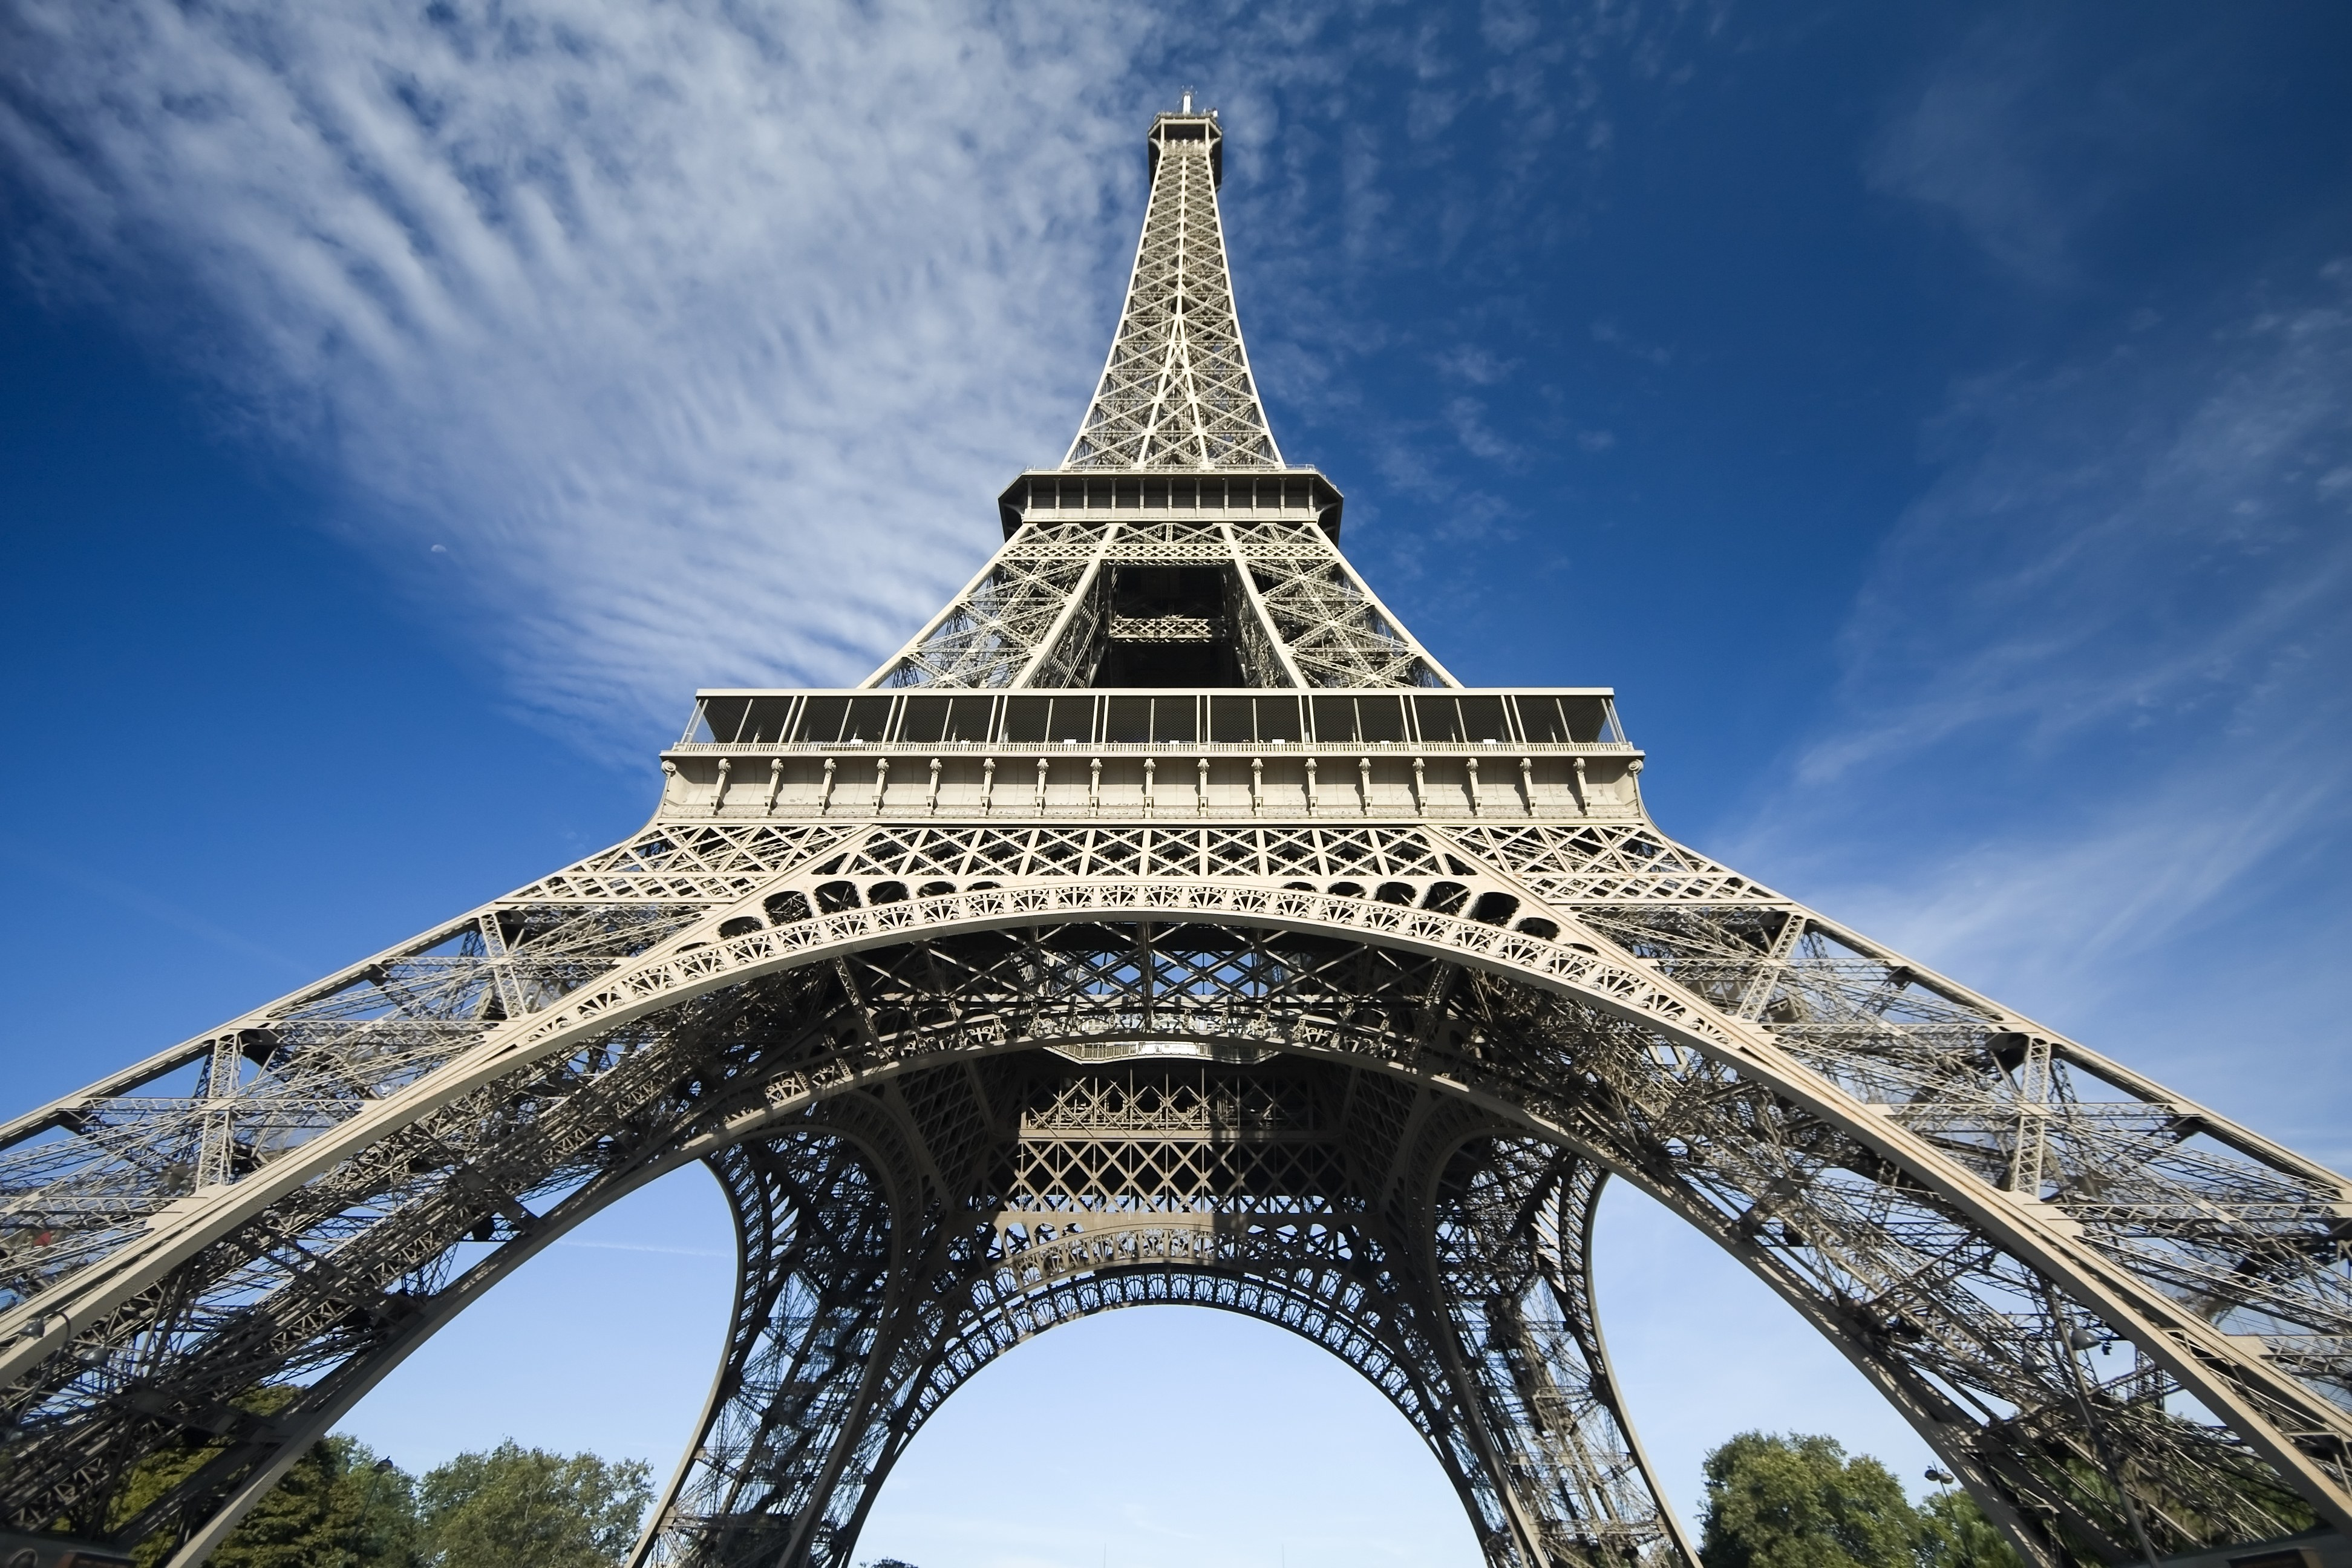
\includegraphics[scale=0.08]{eiffel.jpg}
    \\
    \textit{eiffel.jpg}
\end{center}
\bigskip
\begin{center}
    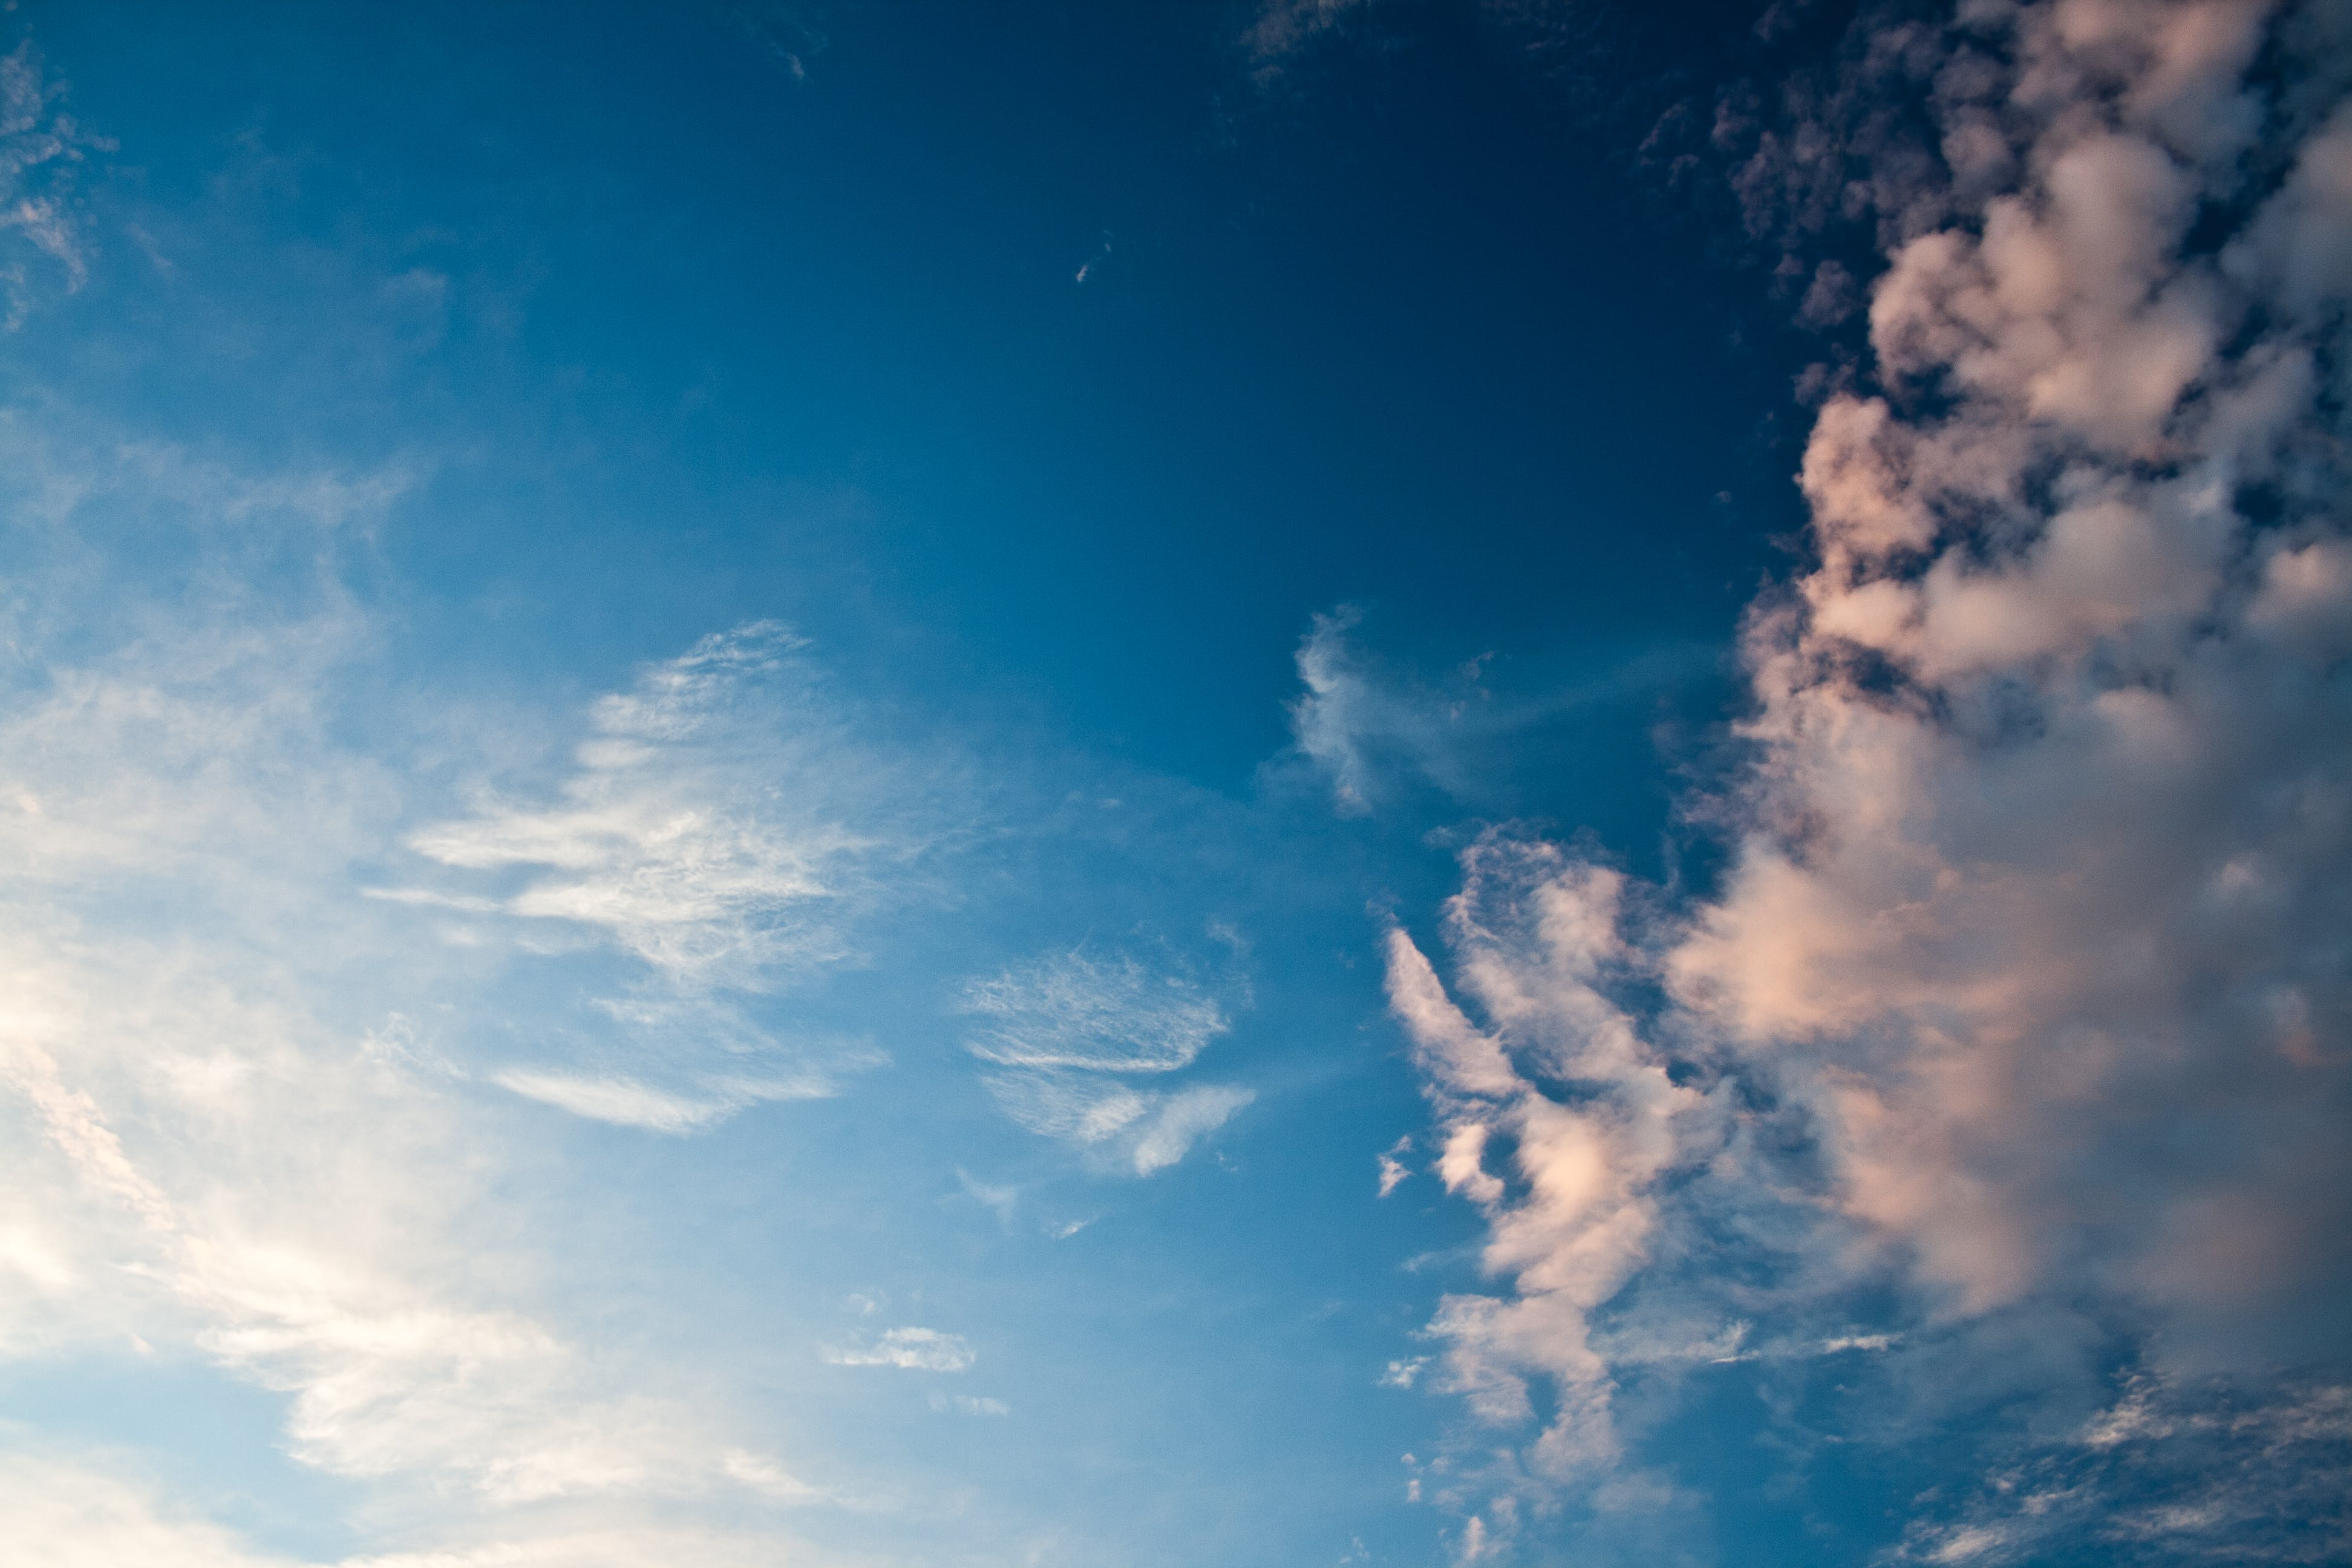
\includegraphics[scale=0.08]{sky.jpg}
    \\
    \textit{sky.jpg}
\end{center}
    


\section{Labwork 6: Map}
This labwork contains 3 sections using map method. Each of them is implemented in a separated kernel with 2D blocks of 32x32 threads on a 2D grid. 
\subsection{Grayscale image binarization}
In this part, each grayscale pixel of the input image is converted to a binary corresponding to black and white. The technique that is applied is thresholding with a threshold number inputed from keyboard. If the grayscale value is greater than the threshold number, it is set equal to 255, otherwise, it is equal to 0.
\\
\begin{lstlisting}[language=C]
unsigned char g = (input[tid].x + input[tid].y 
                    + input[tid].z) / 3;
	if (g>= thresholdnumber){
		g = 255;
	}else{
		g = 0;
	}
    output[tid].z = output[tid].y = output[tid].x = g; 
\end{lstlisting}
\textit{Optimization:} The grayscale value g is stored in the register before calculating so it will be faster.
\\
\begin{center}
    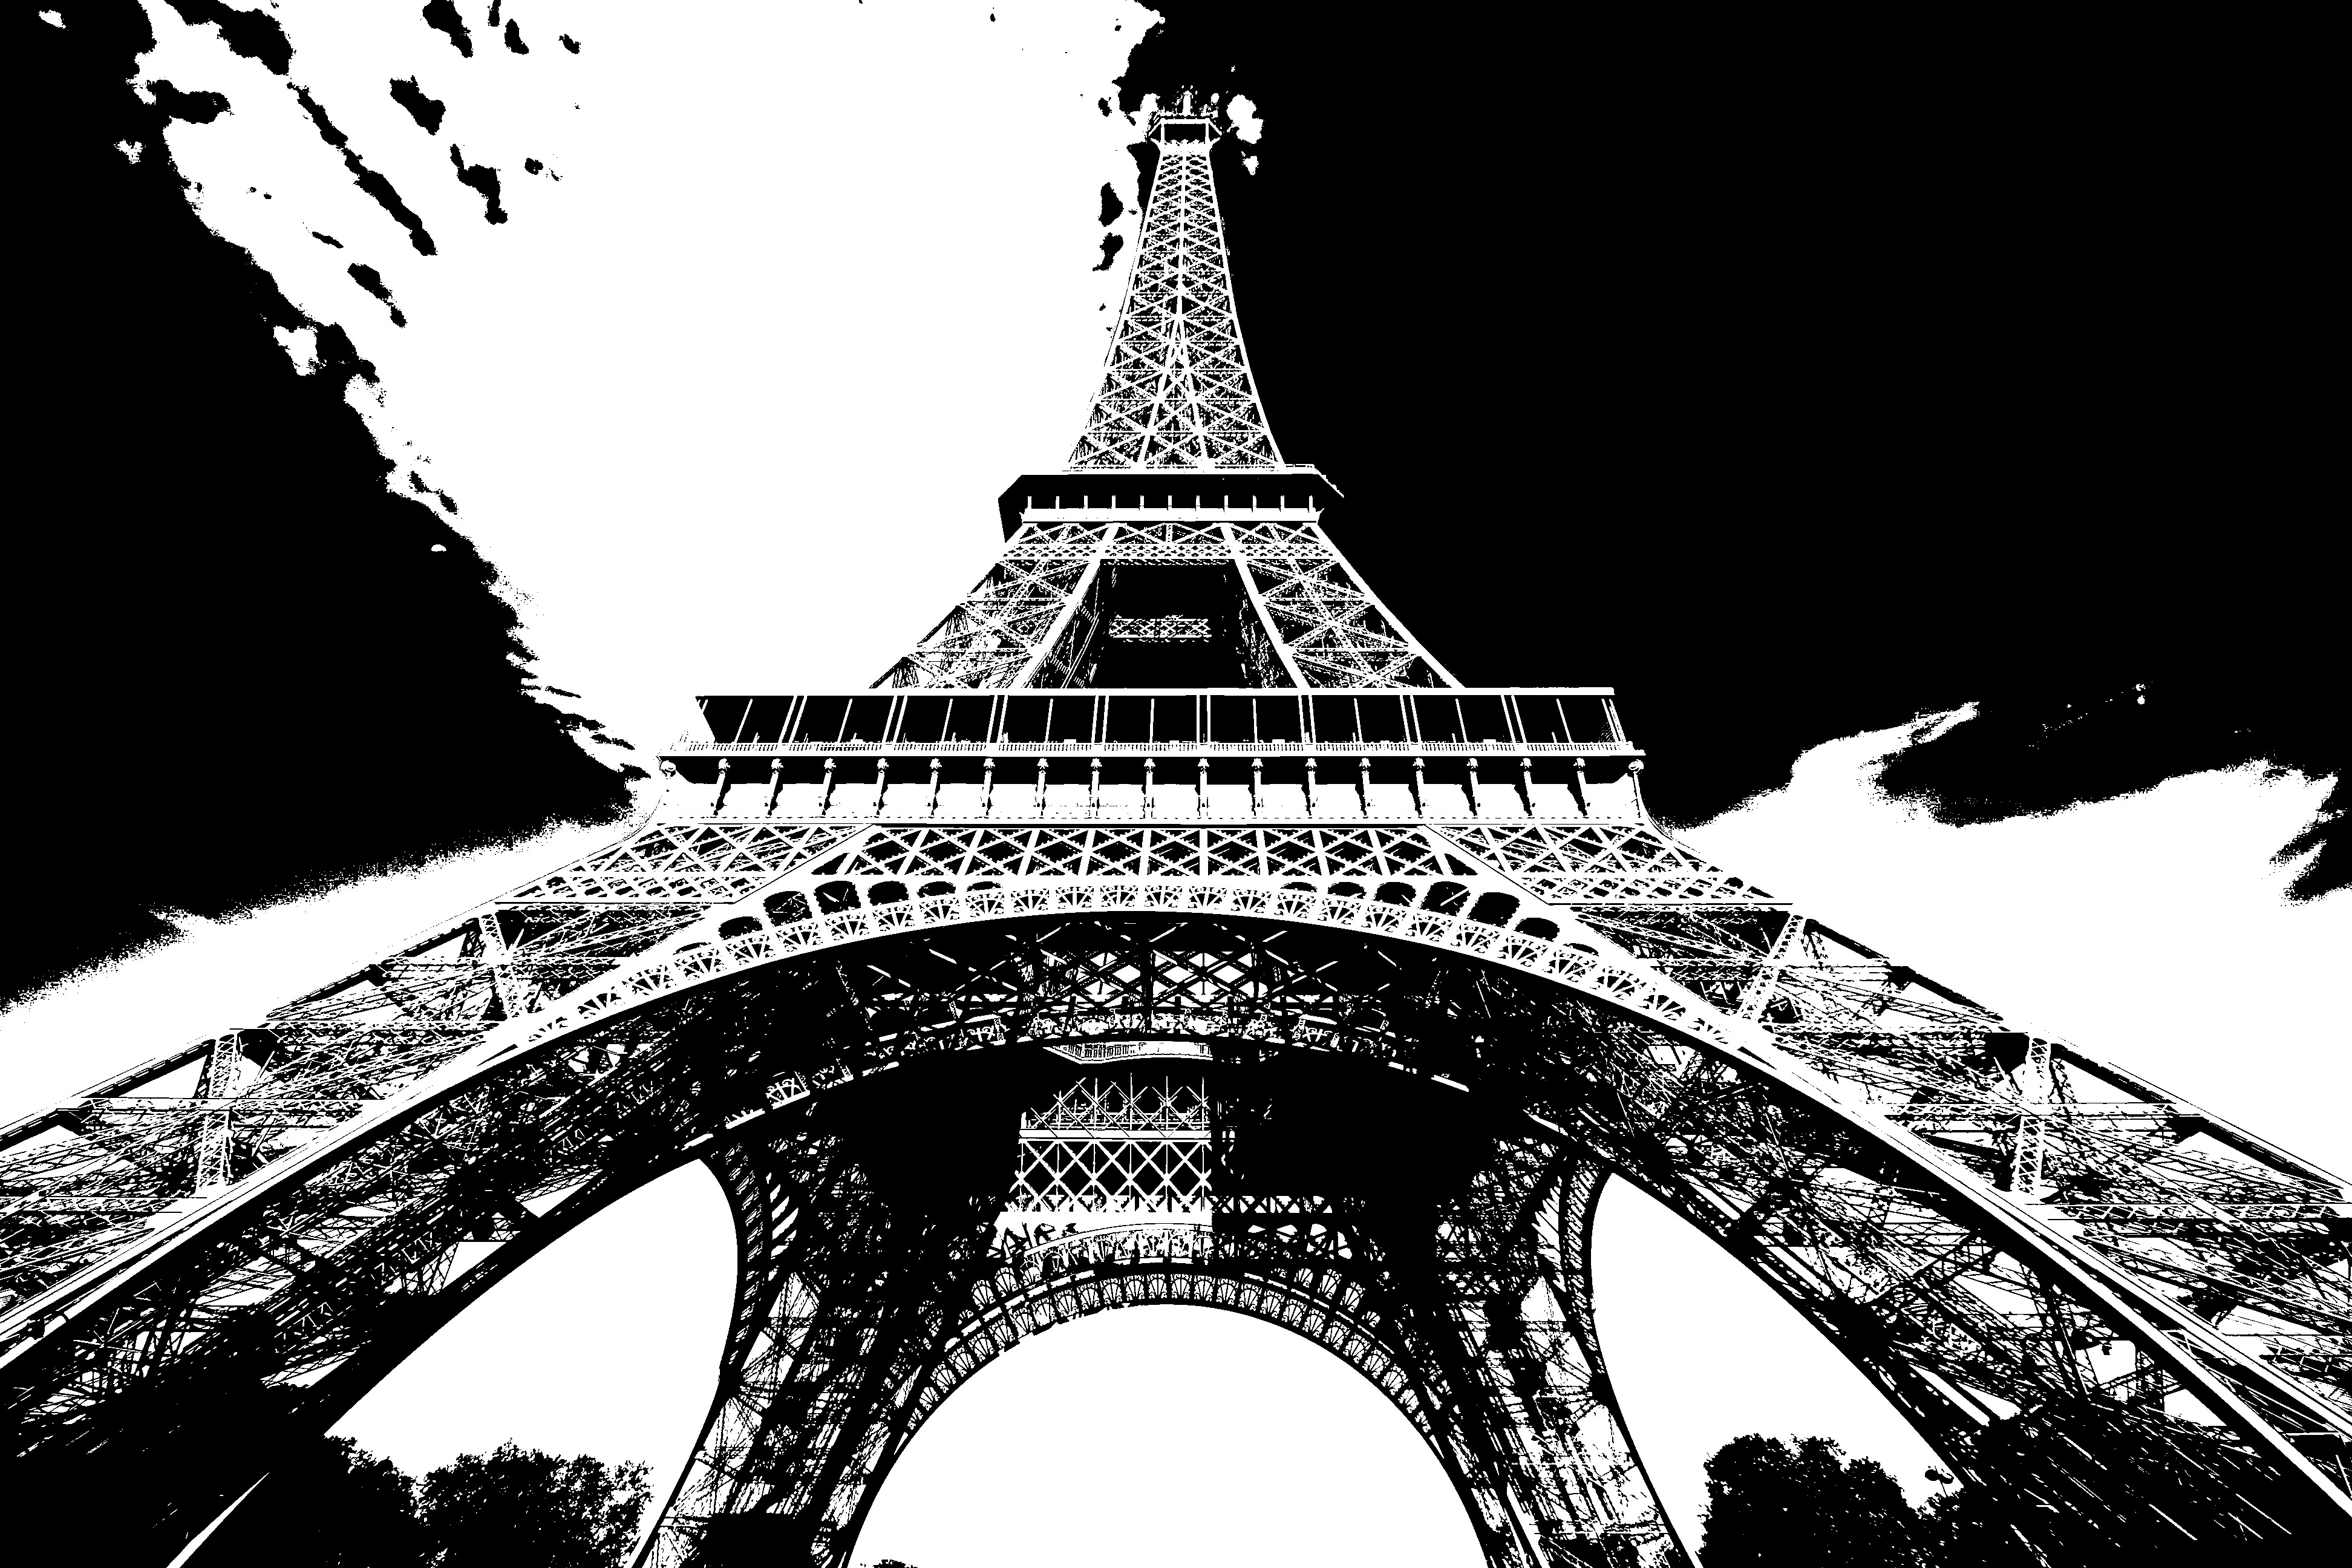
\includegraphics[scale=0.08]{threshold.jpg}
    \\
    \textit{Binarization output with threshold number = 127}
\end{center}

\subsection{Brightness control}
This part is quite similar to the previous one, with a brightness number inputed from keyboard. Then all pixel values are increased by that number. 
\begin{lstlisting}[language=C]
unsigned char g = (input[tid].x + input[tid].y 
                    + input[tid].z) / 3;
	g += brightnessnumber;
    output[tid].z = output[tid].y = output[tid].x = g; 
\end{lstlisting}
\textit{Optimization:} The grayscale value g is stored in the register before calculating so it will be faster.\\

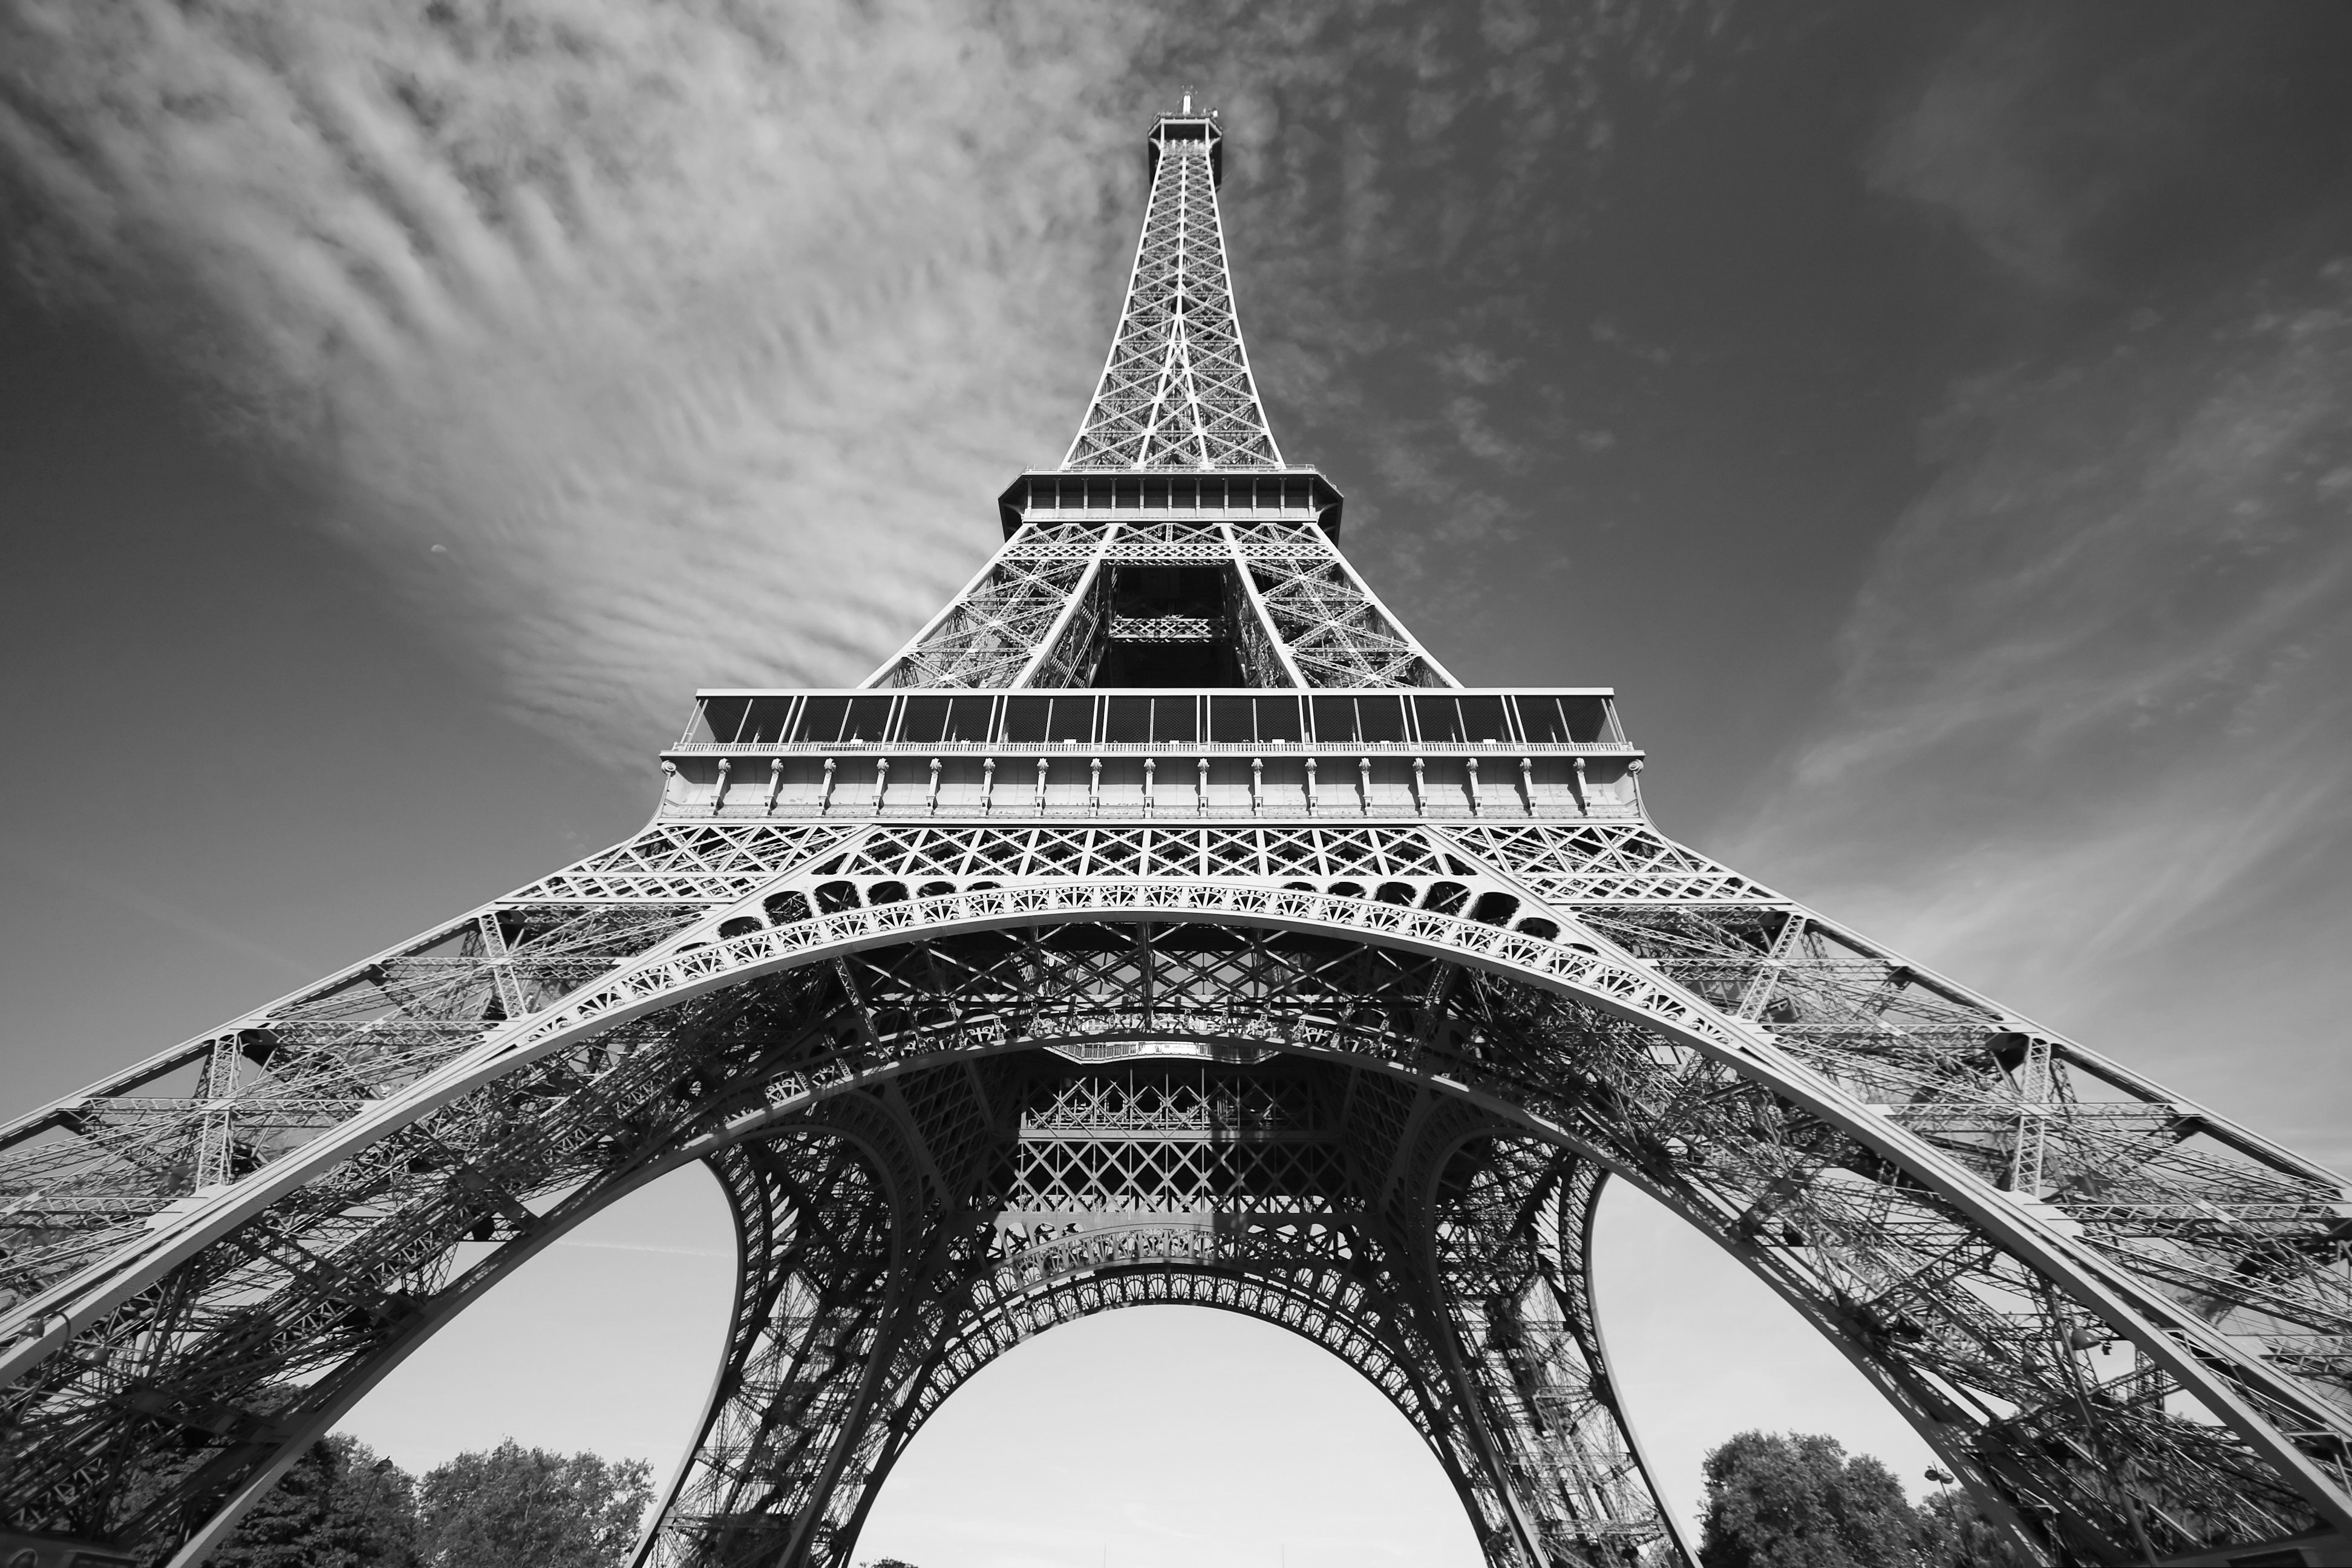
\includegraphics[scale=0.045]{eiffelGray.jpg}
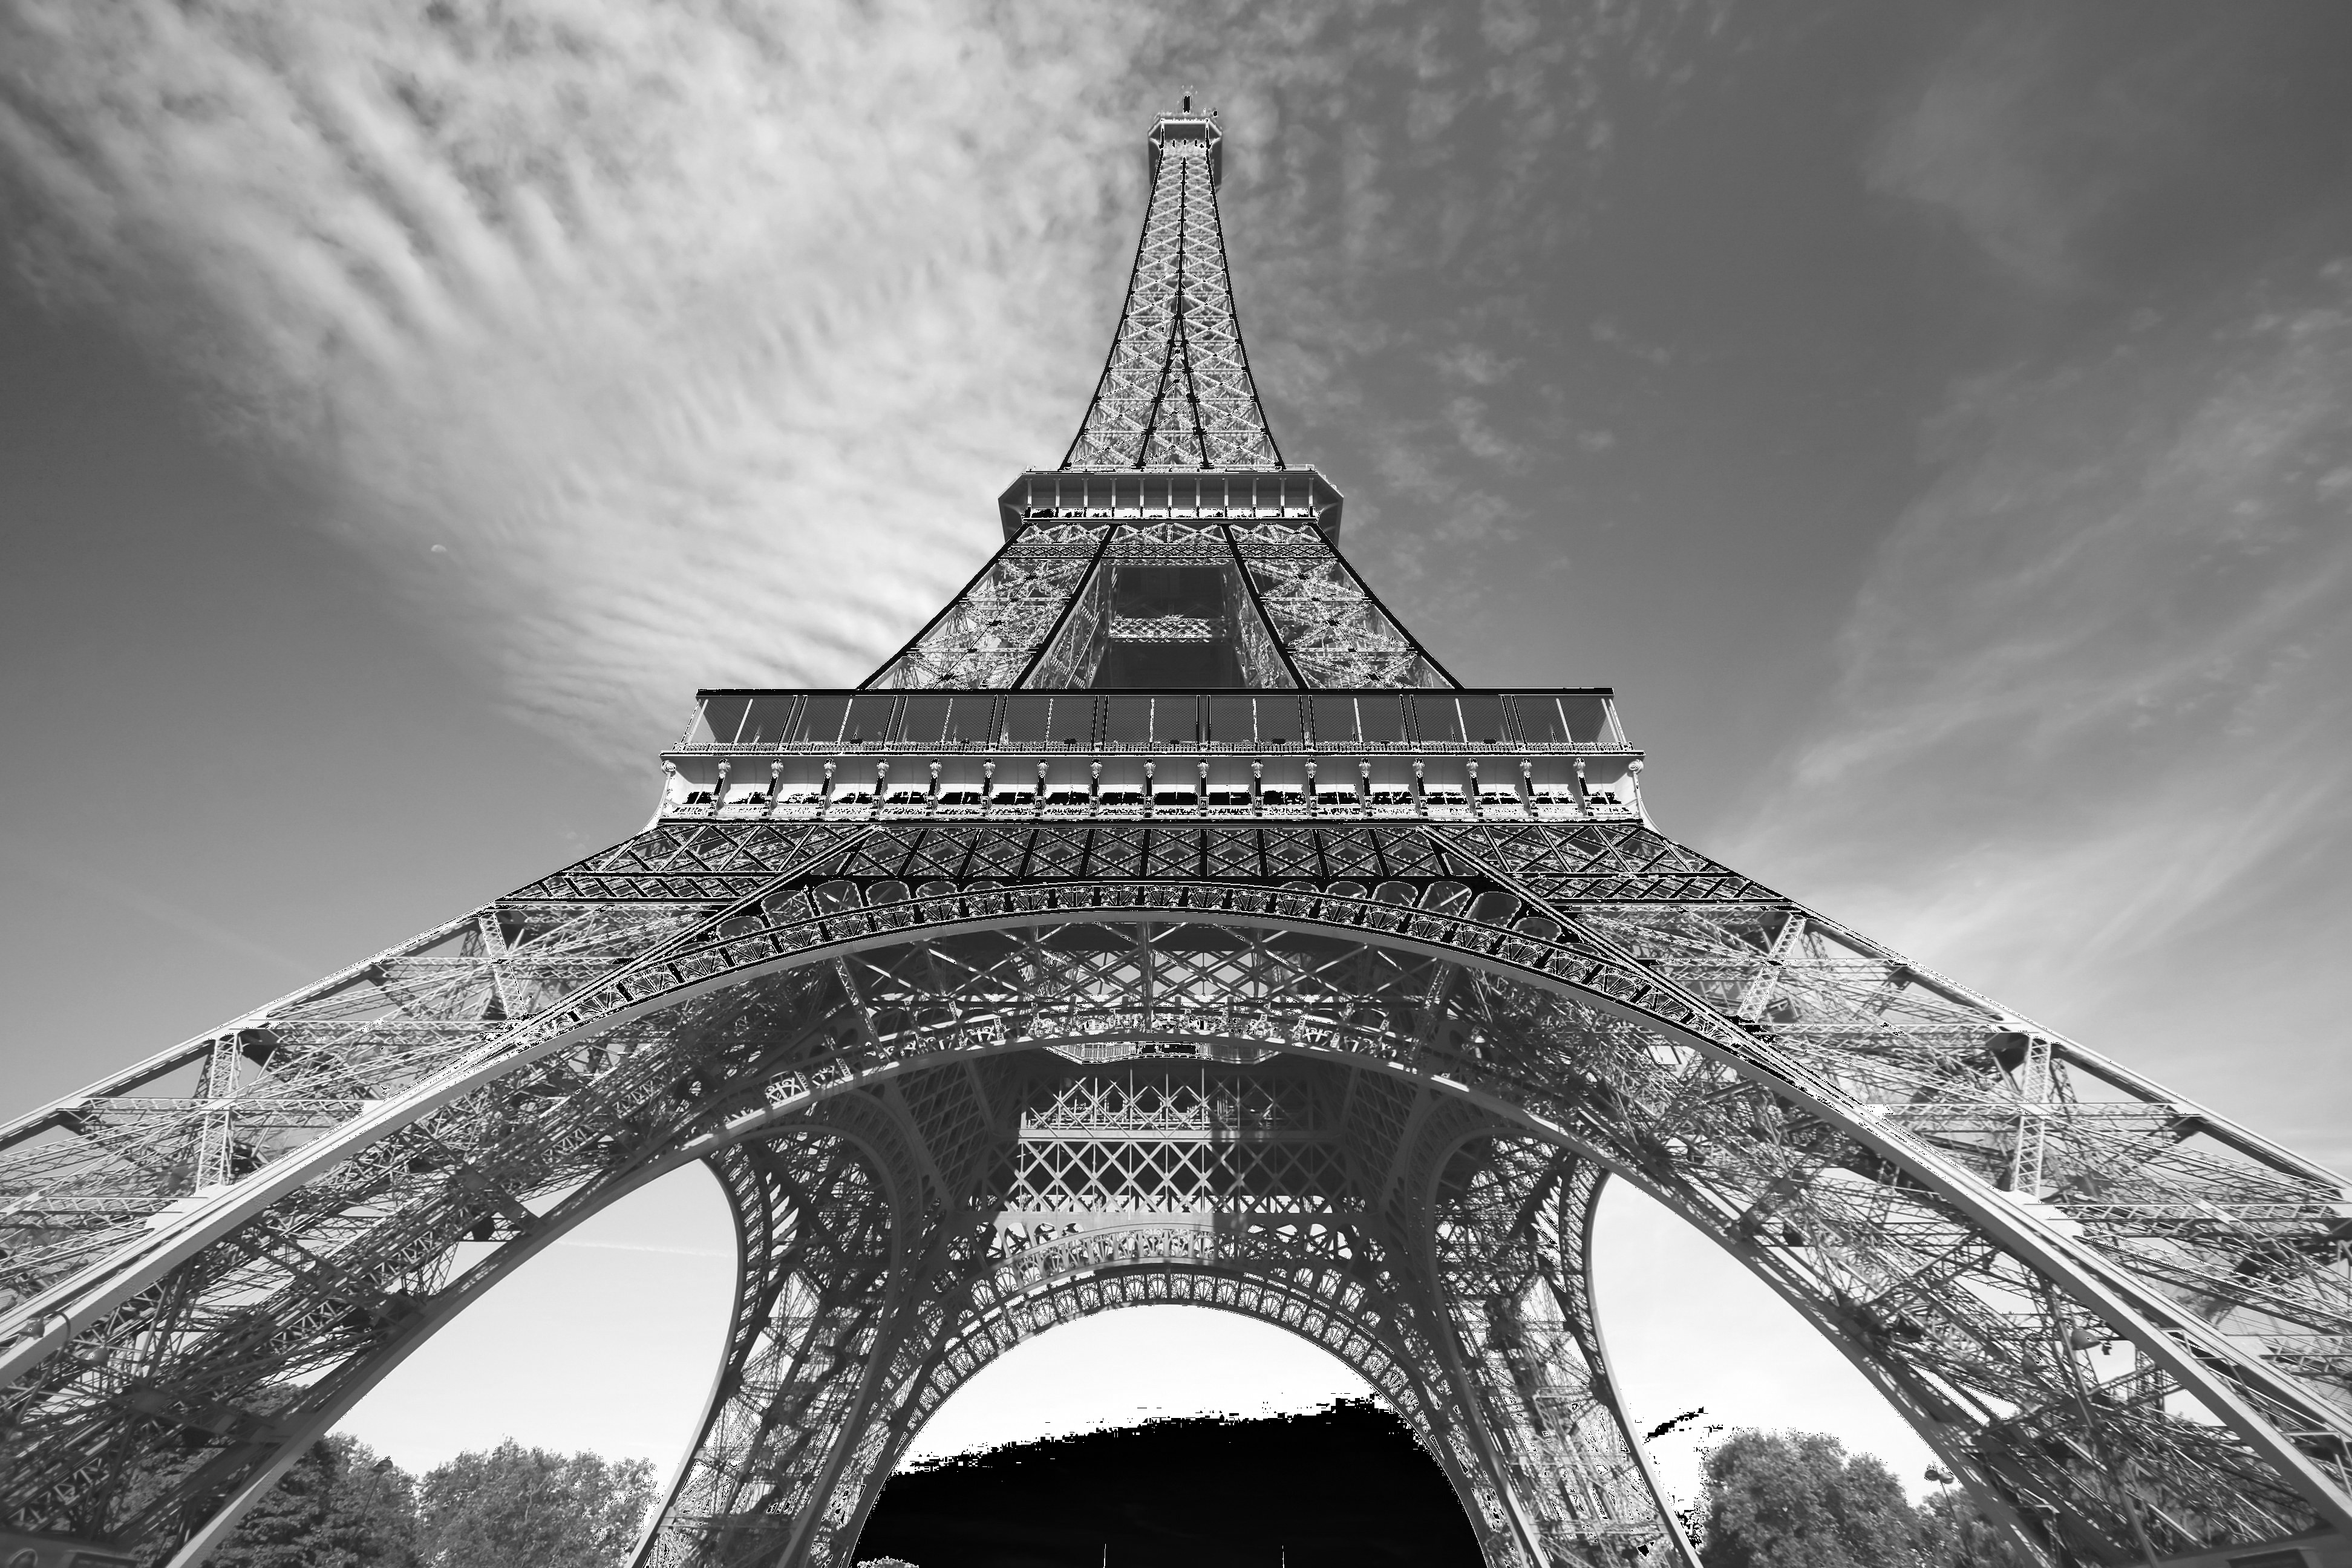
\includegraphics[scale=0.045]{brightness.jpg}\\
\textit{Original grayscale image (left) and graycale one with brightness increased by 30 (right)}

\subsection{Blending two images}
Two image eiffel.jpg and sky.jpg having the same size are combined together with a inputed coefficient defining the "weight" of each image. The task is applied with both color images and grayscale images.
\subsubsection{Color image}
\begin{lstlisting}[language=C]
    output[tid].x = (weight * (double)input[tid].x) 
                + ((1.0 - weight) * (double)input2[tid].x);
    output[tid].y = (weight * (double)input[tid].y) 
                + ((1.0 - weight) * (double)input2[tid].y);
    output[tid].z = (weight * (double)input[tid].z) 
                + ((1.0 - weight) * (double)input2[tid].z);
\end{lstlisting}

\begin{center}
    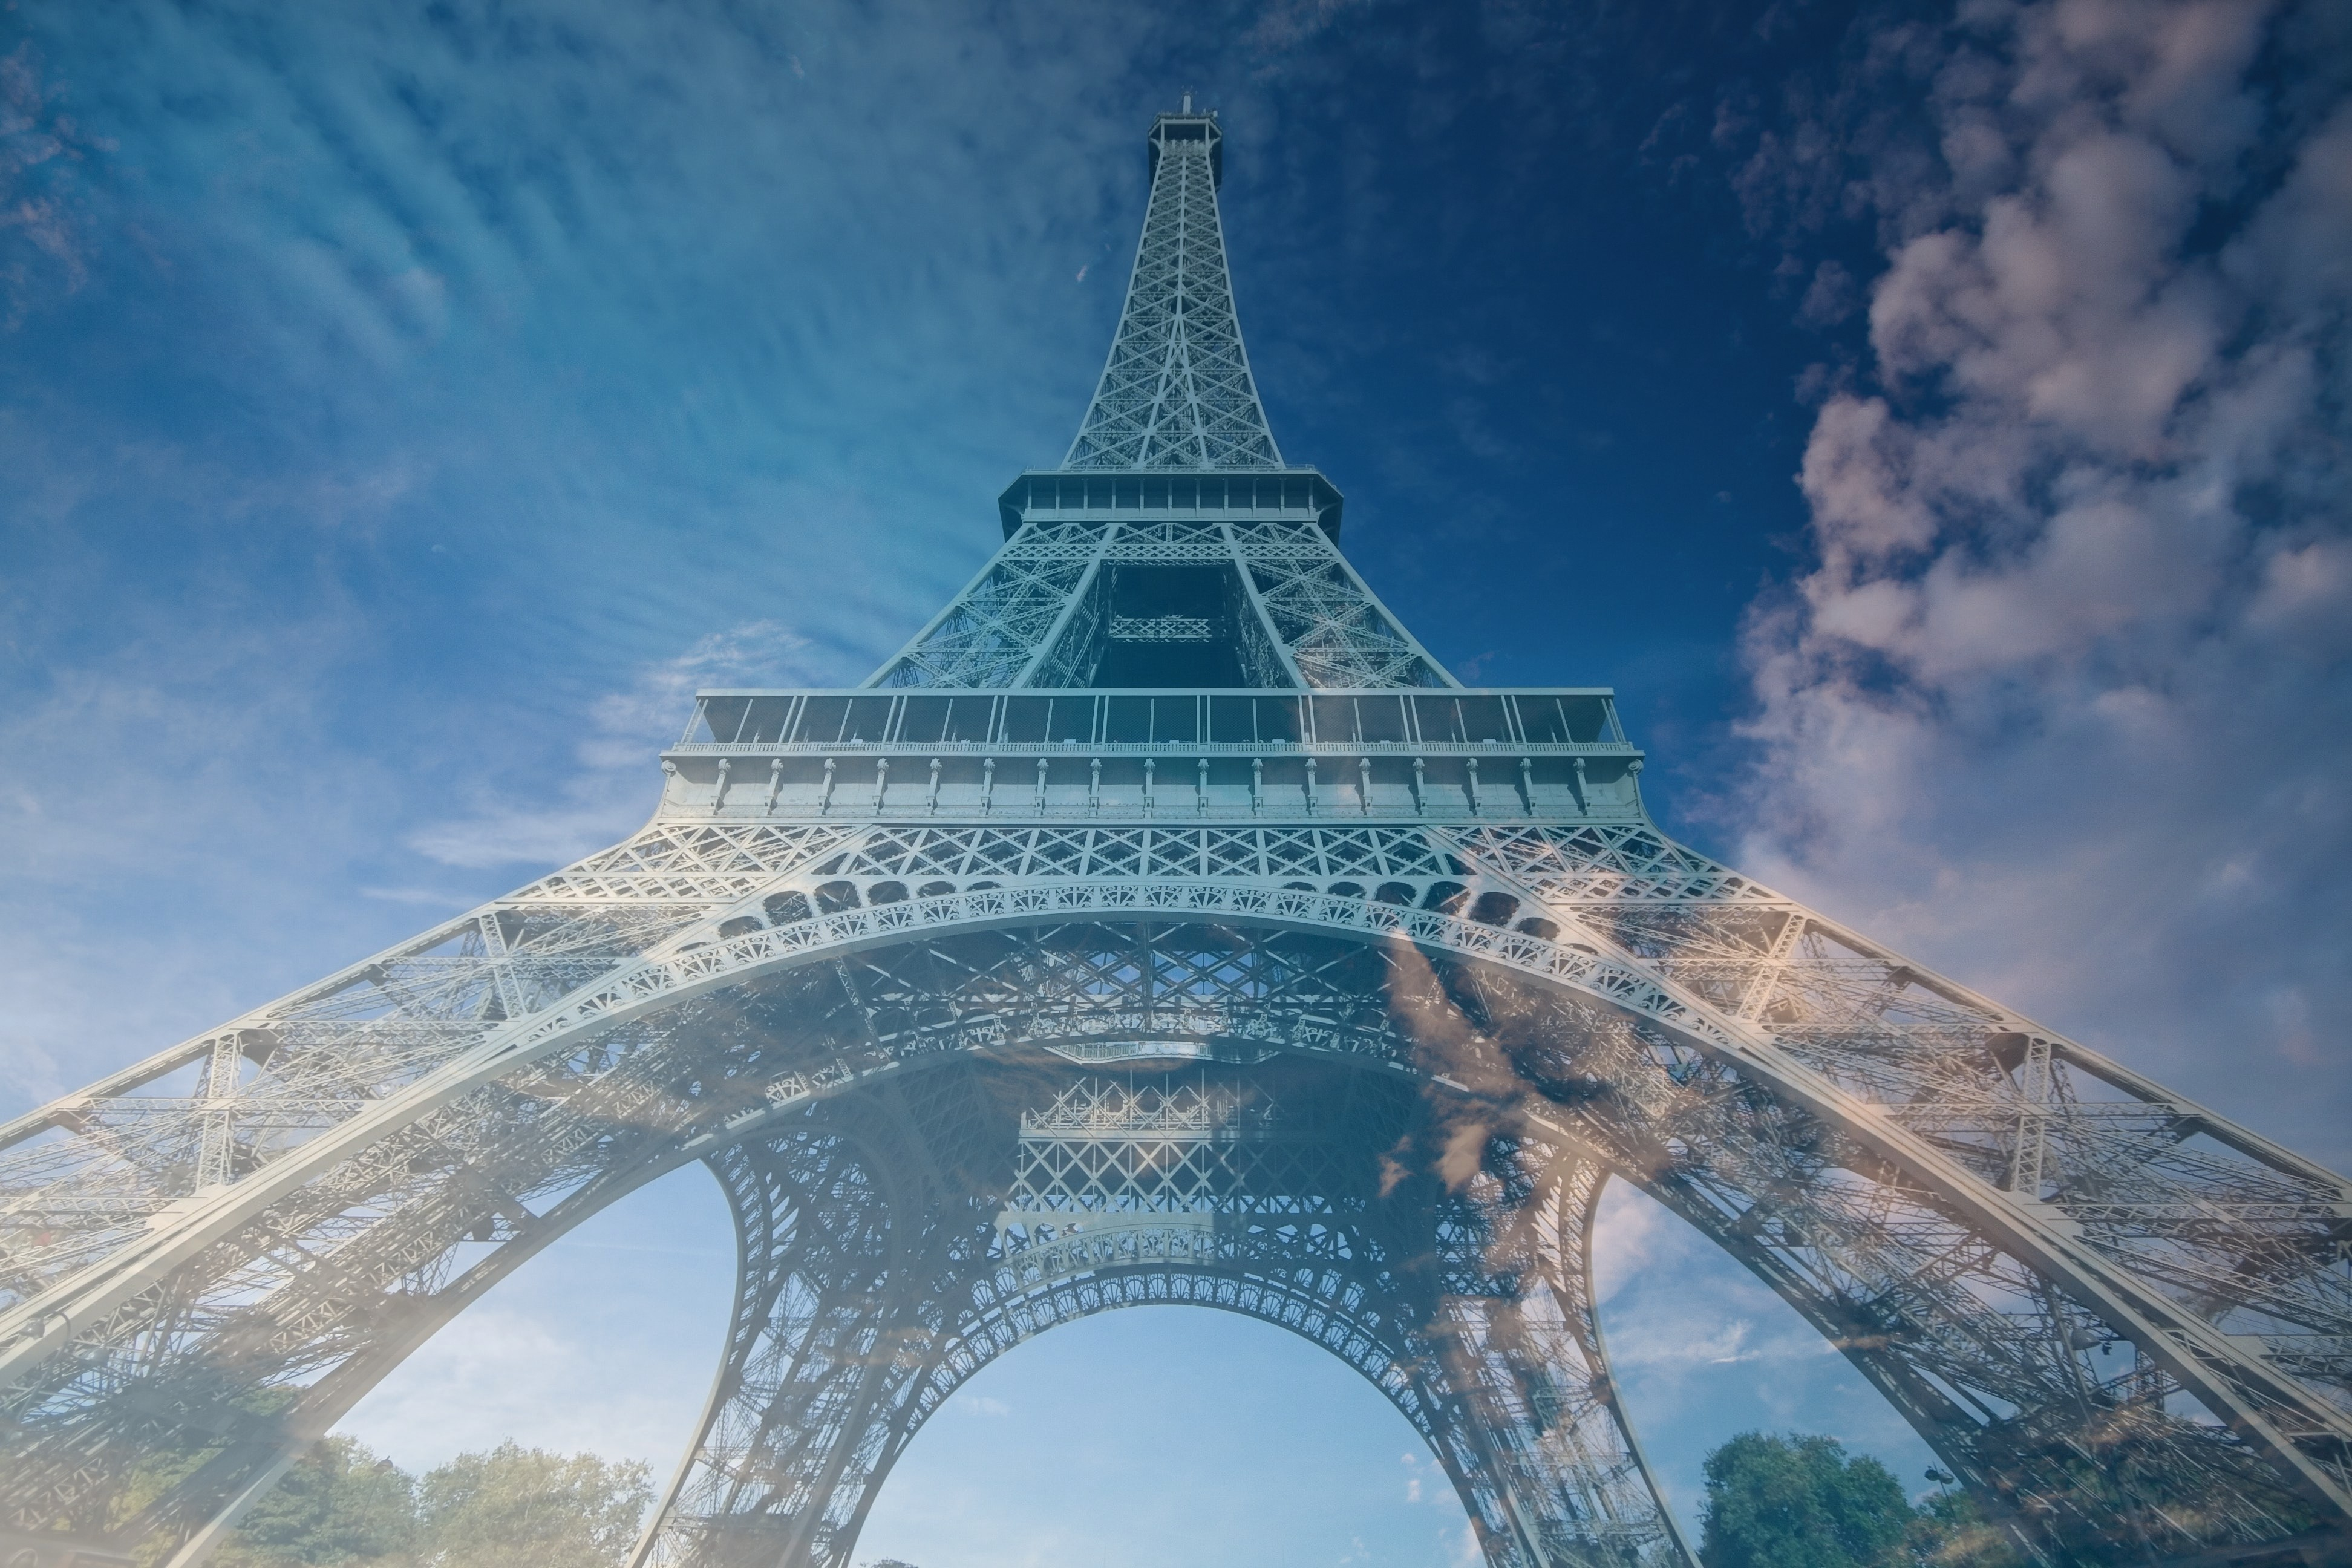
\includegraphics[width=\linewidth]{blendingrgb.jpg}
    \\
    \textit{Blending applied with color images with coefficient = 3}
\end{center}

\subsubsection{Grayscale image}
\begin{lstlisting}[language=C]
    unsigned char g = (input[tid].x + input[tid].y 
                        + input[tid].z) / 3;
    unsigned char g2 = (input2[tid].x + input2[tid].y 
	                    + input2[tid].z) / 3;
	g = weight*g + (1.0-weight)*g2;
    output[tid].z = output[tid].y = output[tid].x = g; 
\end{lstlisting}
\textit{Optimization:} The grayscale value g is stored in the register before calculating so it will be faster.
\\

\begin{center}
    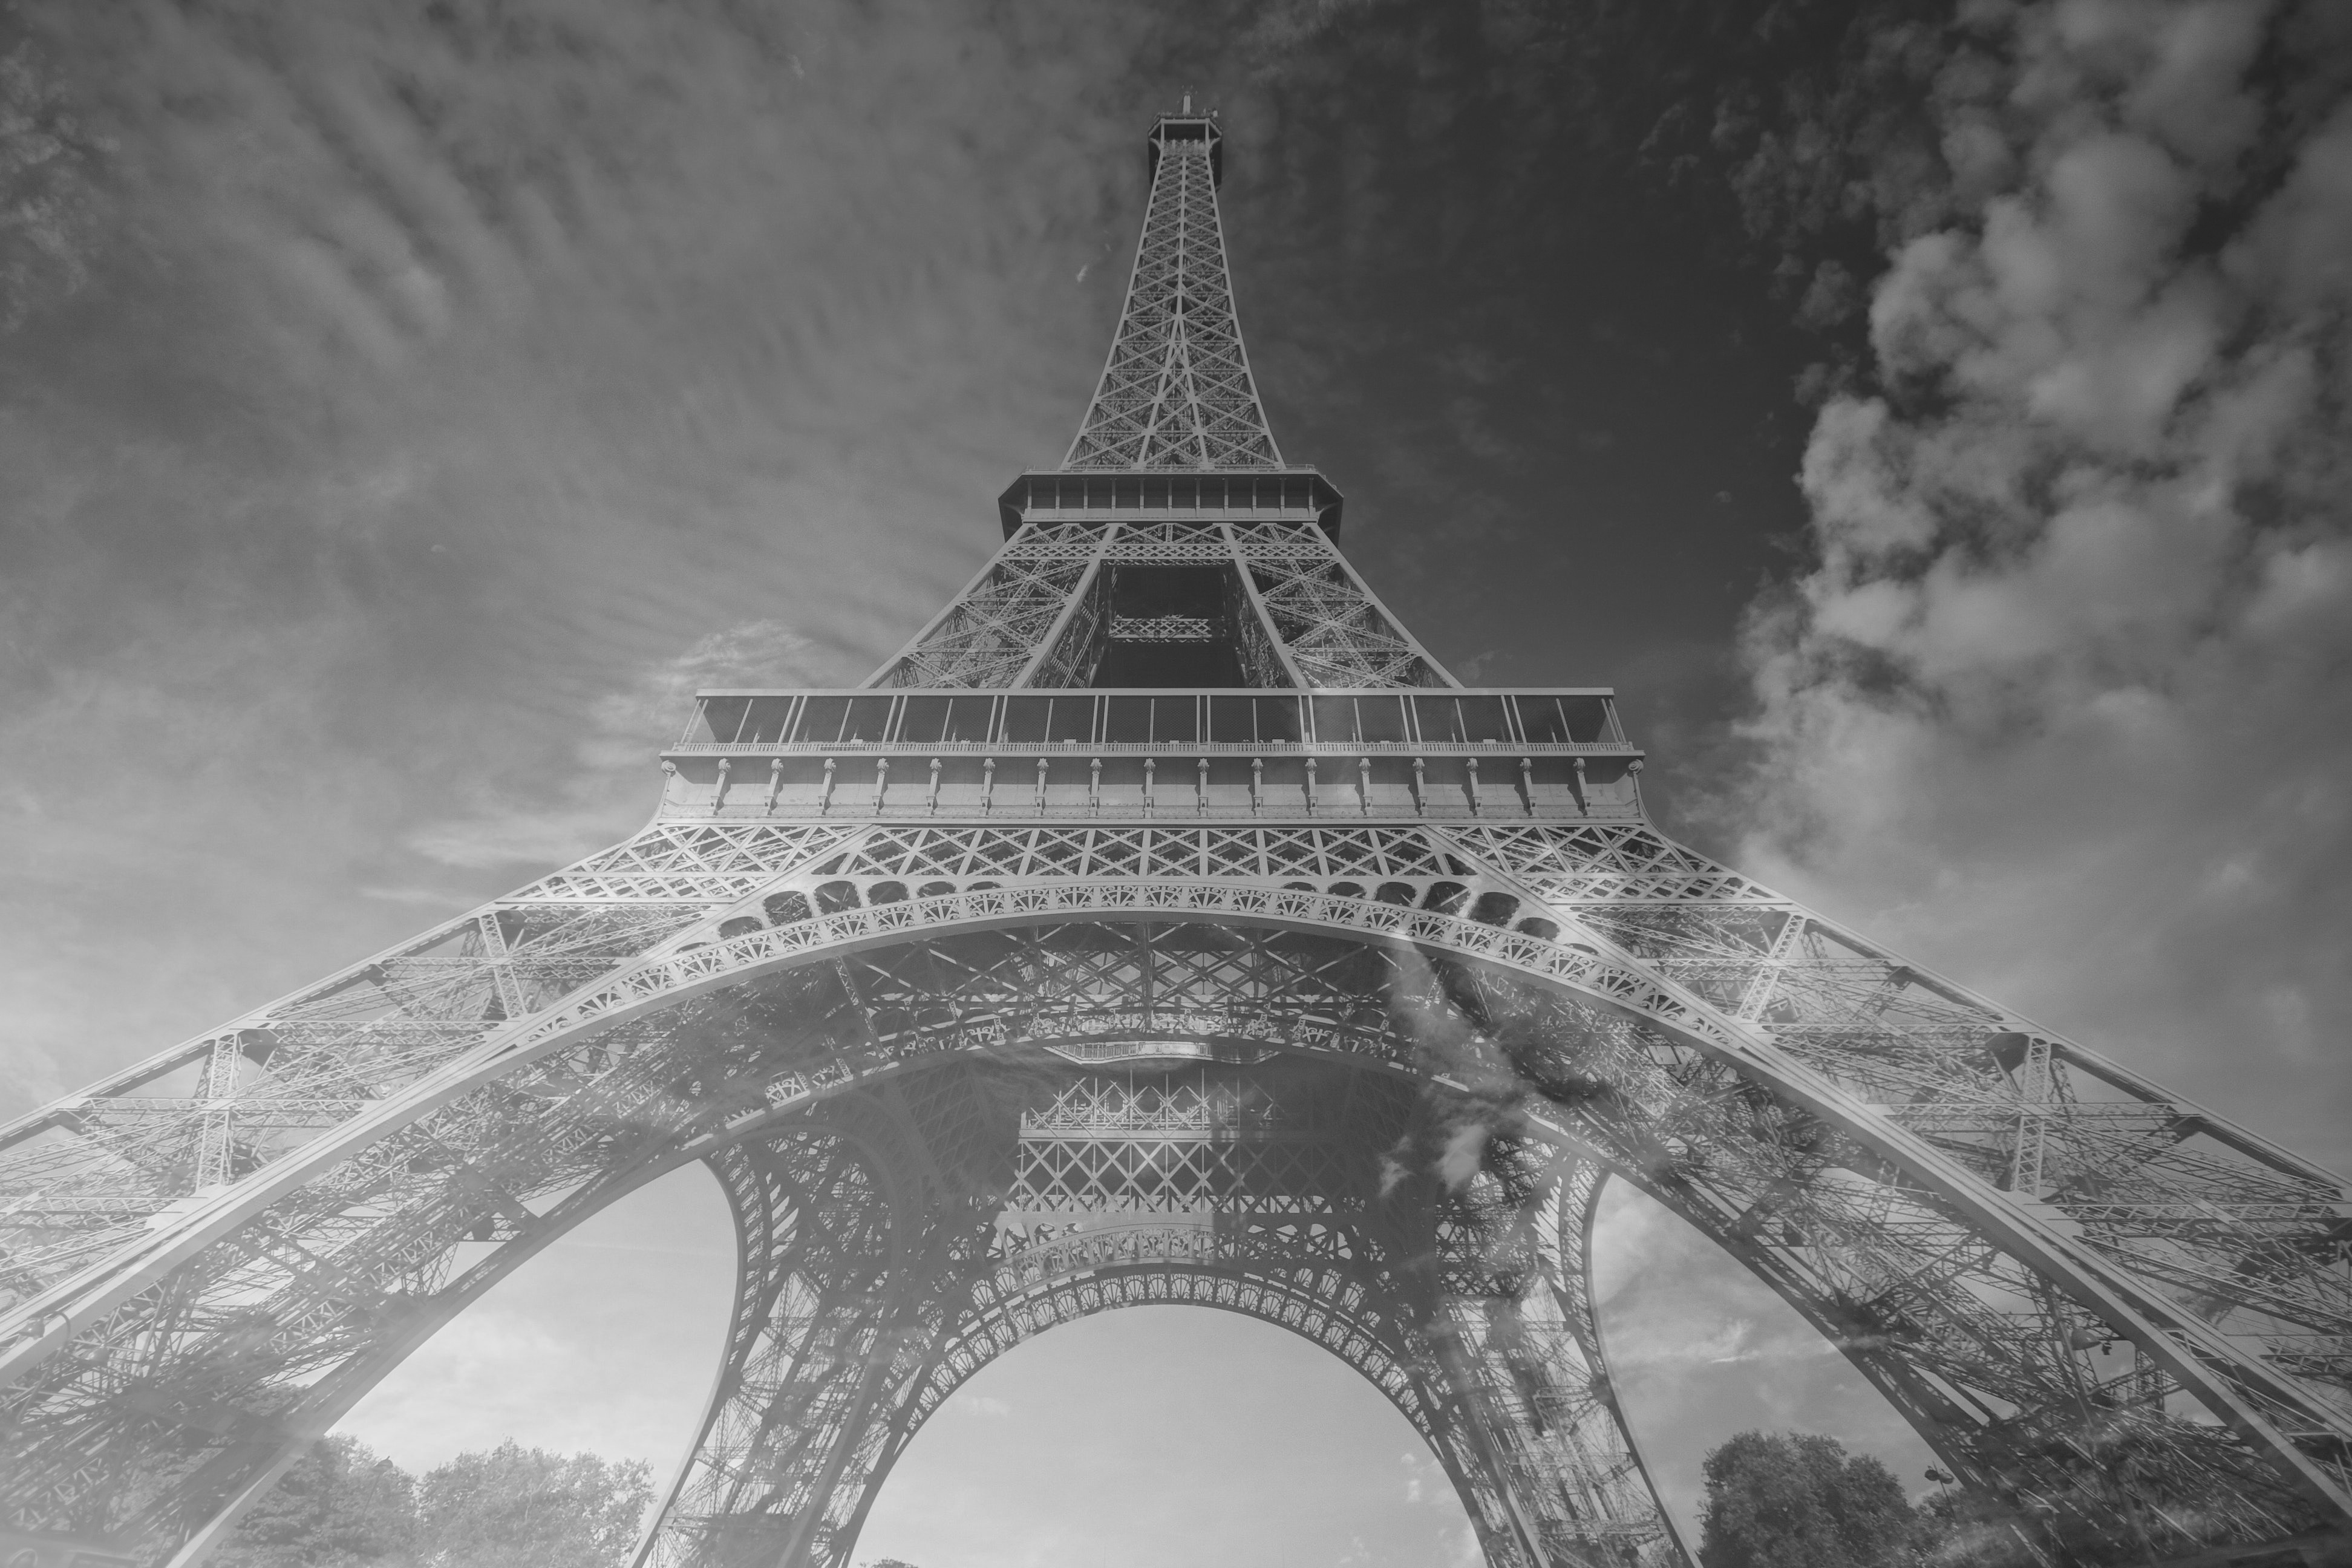
\includegraphics[width=\linewidth]{blendinggray.jpg}
    \\
    \textit{Blending applied with grayscale images with coefficient = 3}
\end{center}

\section{Labwork 7: Reduction}
This labwork linearly recalculates intensity for each pixel in the grayscale image by stretching it. \\

The first task is to find the max and min intensity of the image using reduction after converting it to the grayscale one.

\begin{lstlisting}[language=C]
grayscale<<<numBlock, blockSize>>>(devInput, tempOutput);
grayscaletoint<<<numBlock, blockSize>>>(tempOutput, devMin,
            devMax, inputImage->width, inputImage->height);
reduceMinFinal<<<numBlock, blockSize>>>(devMin);
reduceMaxFinal<<<numBlock, blockSize>>>(devMax);
stretching<<<numBlock, blockSize>>>(tempOutput, devOutput,
            minValue[0],  maxValue[0]);
\end{lstlisting}

Finally that pair of [min,max] is stretched to [0,255] by the equation below and the output is produced.
\begin{equation}
    g' = \frac{g - min}{max -min} *255
\end{equation}
\begin{lstlisting}
stretching<<<numBlock, blockSize>>>(tempOutput, devOutput,
            minValue[0],  maxValue[0]);
\end{lstlisting}

The intensity of the grayscale eiffel image has the min and max value are 3 and 255. It is difficult to observe the difference after stretching. The sky one is better, its min value is 21 and max is 178. 

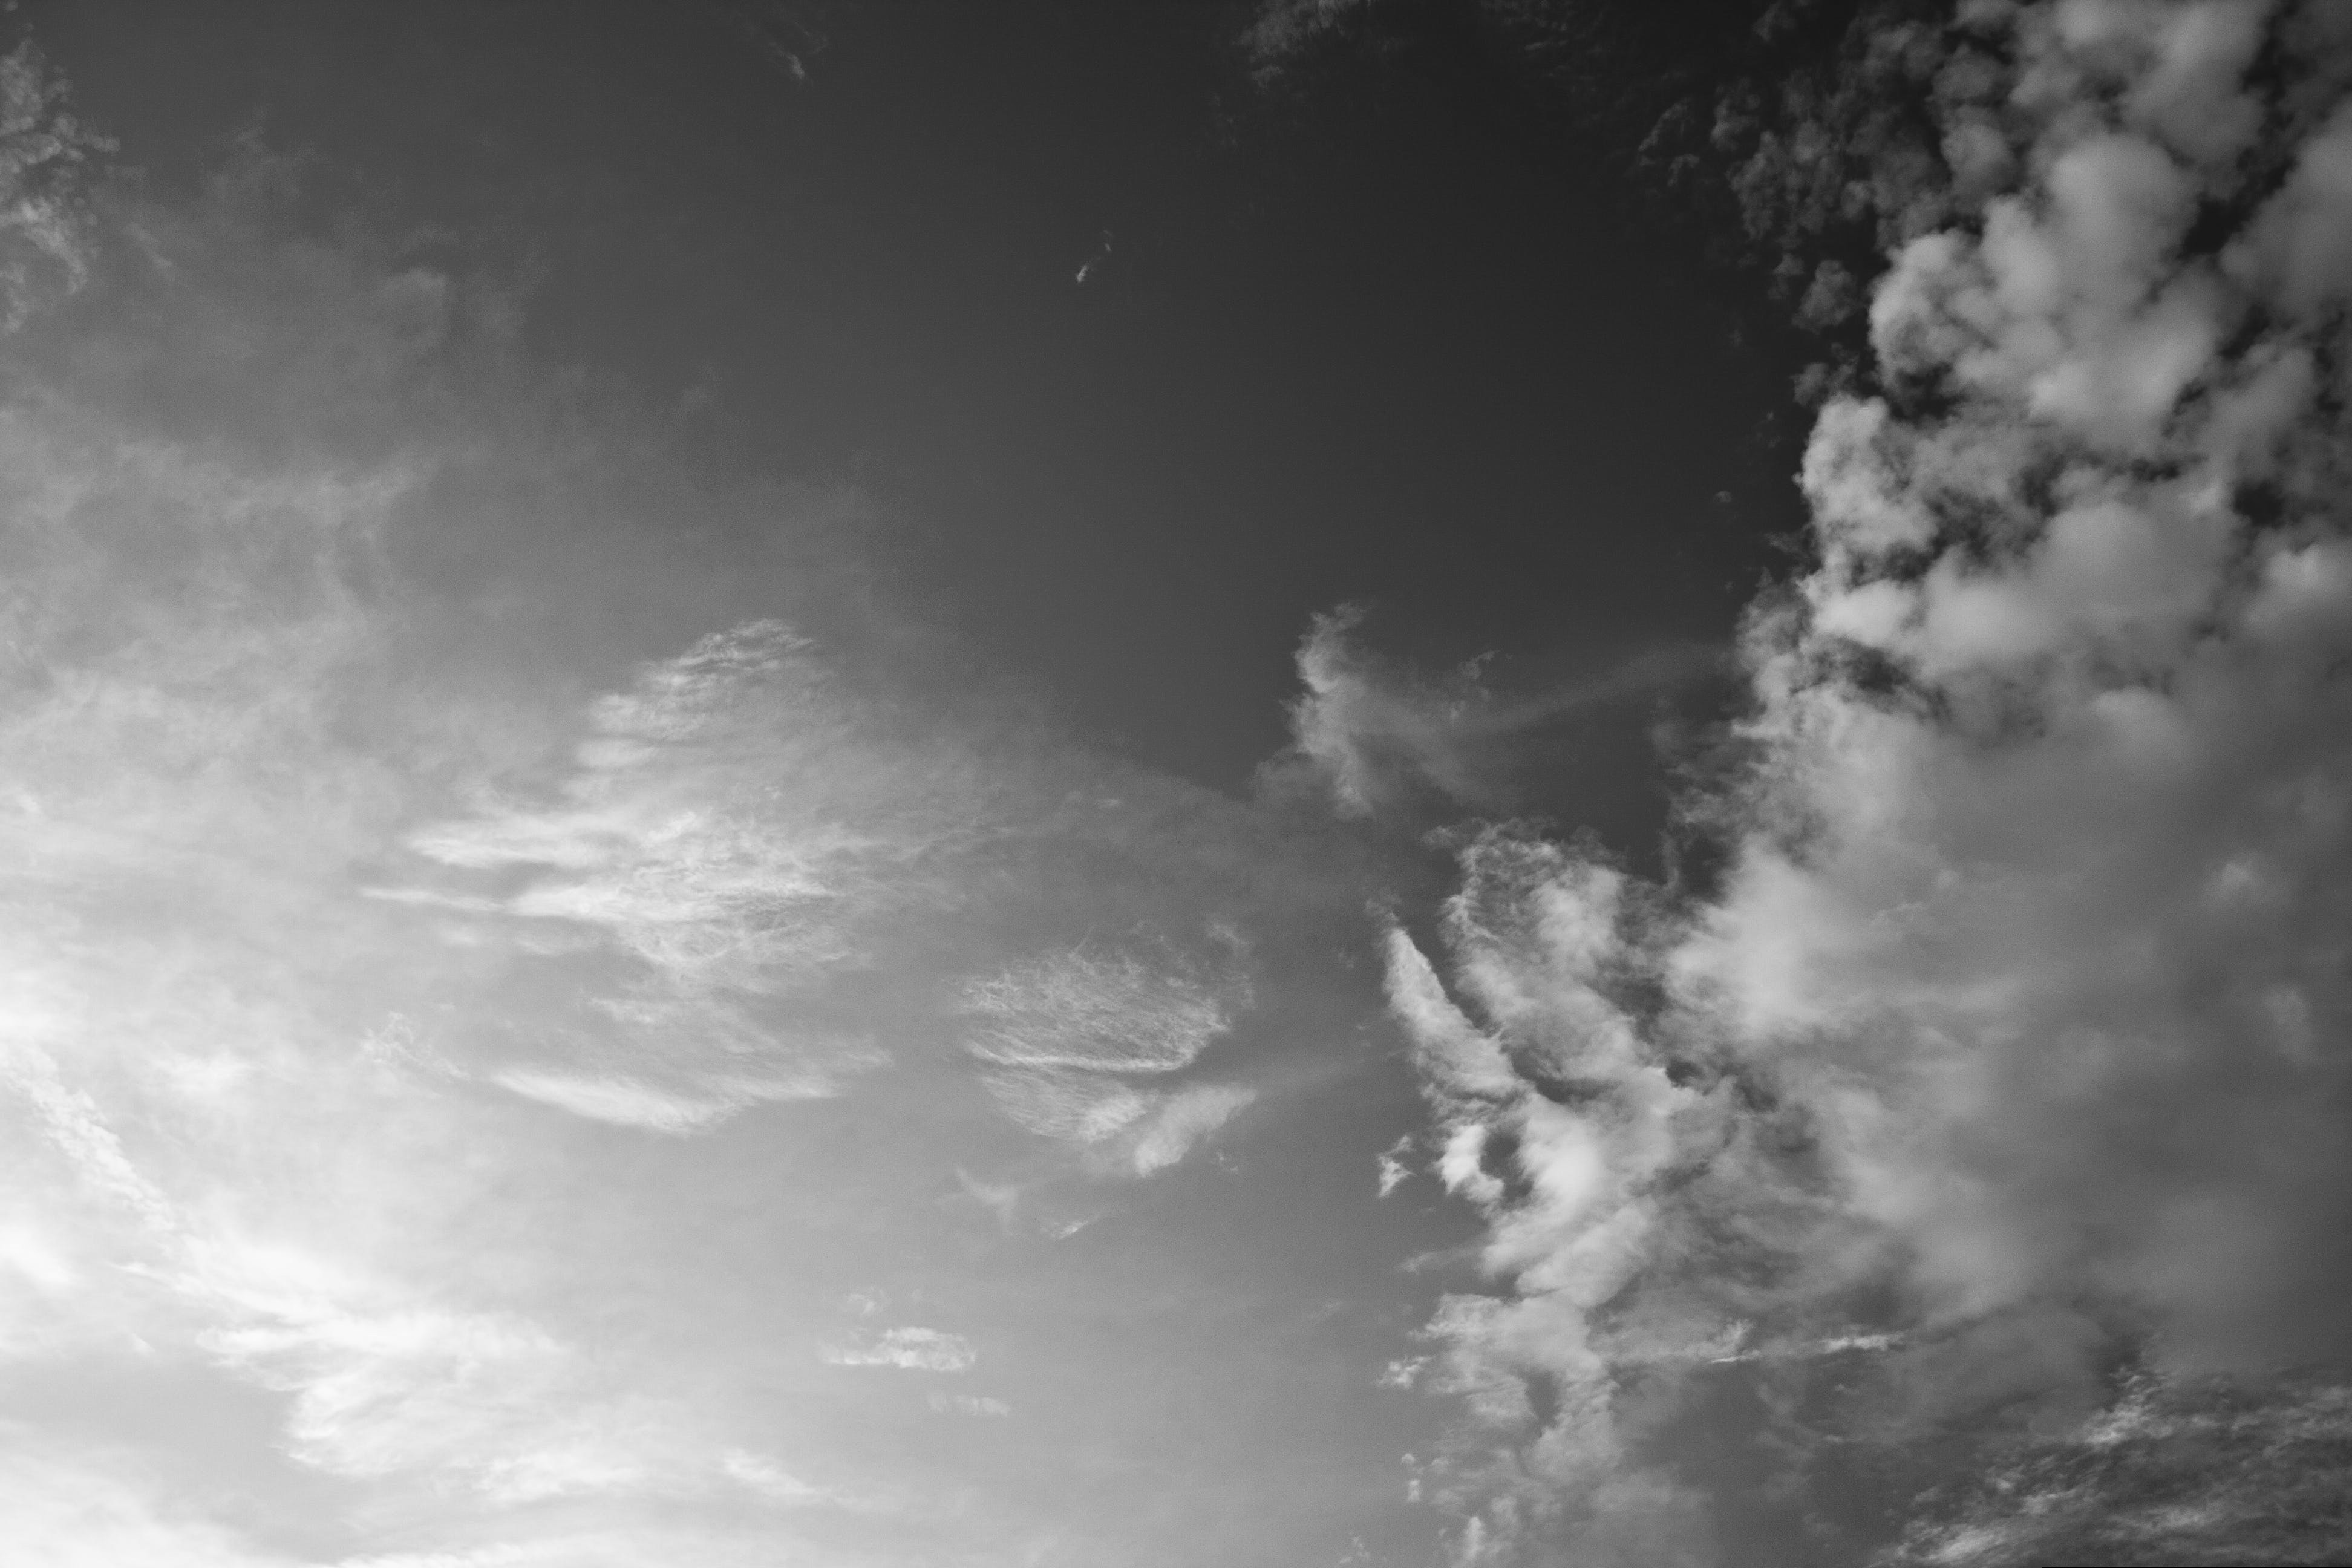
\includegraphics[scale=0.045]{skyGray.jpg}
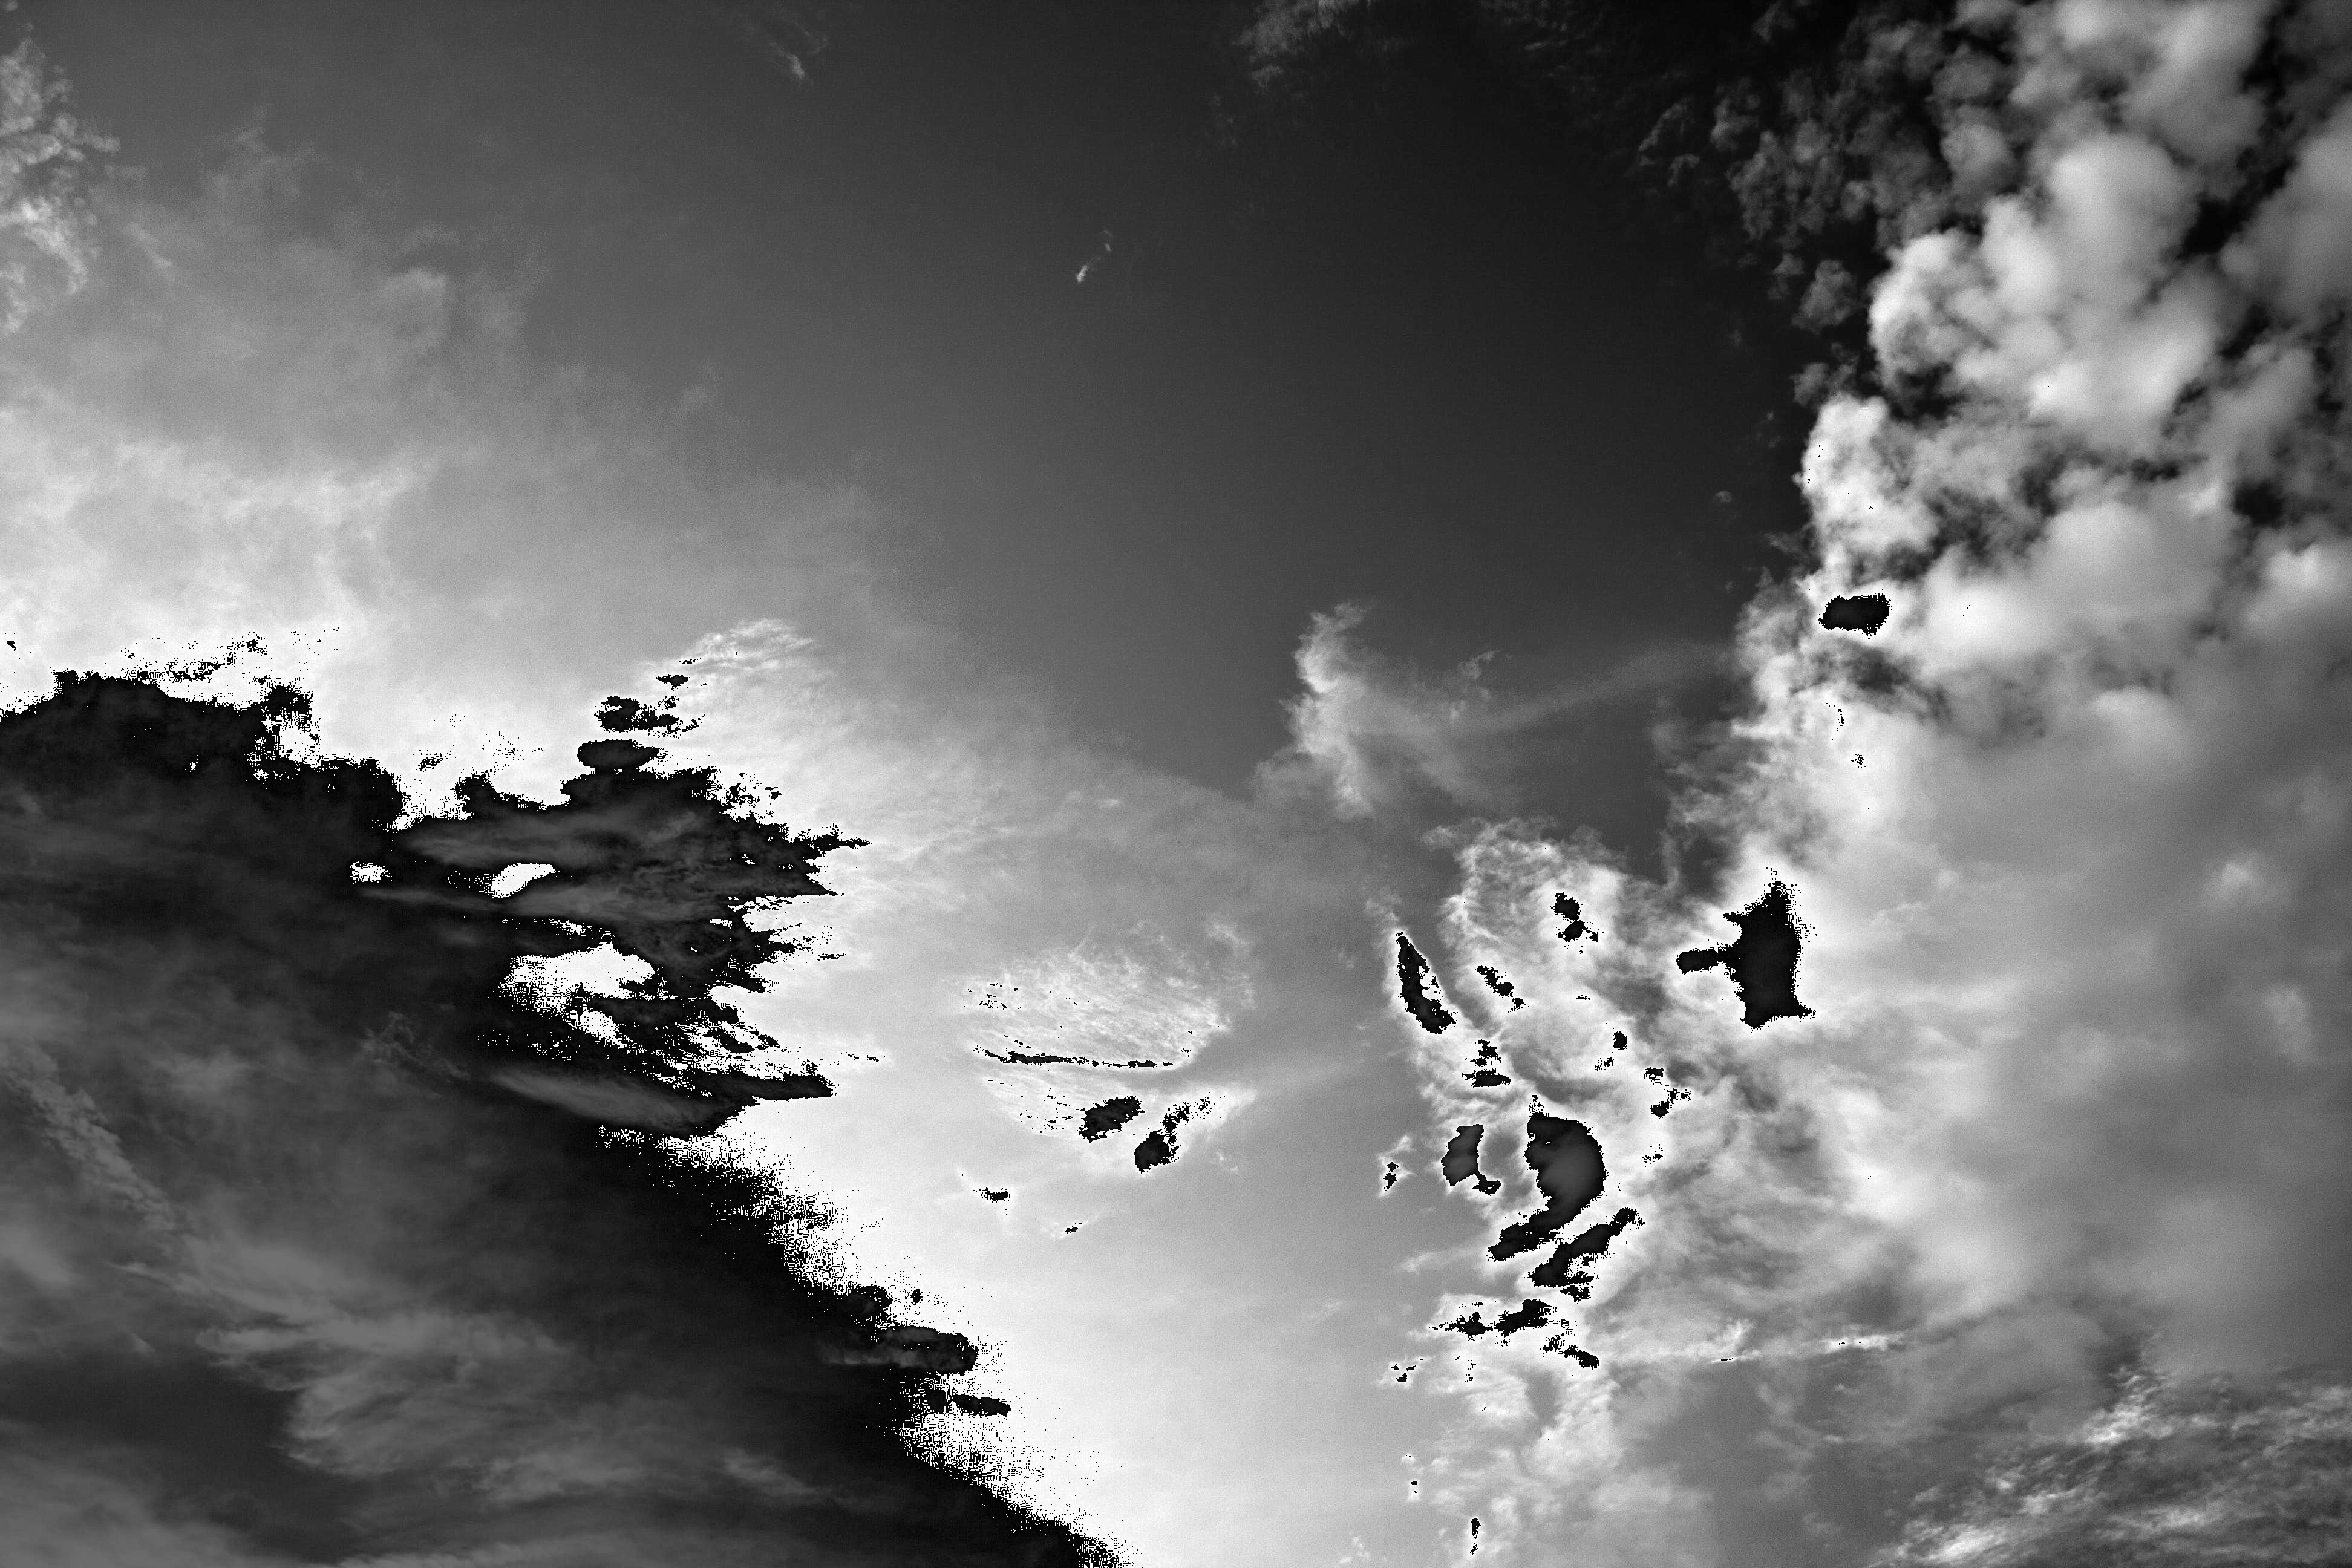
\includegraphics[scale=0.045]{labwork7-gpu-out.jpg}\\
\textit{Original grayscale image (left) and the one after stretching (right}

\section{Labwork 8: Scatter}
In this labwork, the image is firstconverted from RGB to HSV  - array of struct (AoS) to struct of array (SoA).

\begin{lstlisting}[language=C]
struct hsv{
	double *h, *s, *v;
};
\end{lstlisting} 
Then in the second one, the previous result is converted back to RGB channels (SoA to AoS).\\

Each part is implemented in a different kernel with 2D blocks of 32x32 threads on a 2D grid.

\begin{lstlisting}
    rgb2hsv<<<gridSize, blockSize>>>(devInput, devHSV, 
        inputImage->width, inputImage->height);
    hsv2rgb<<<gridSize, blockSize>>>(devHSV, devOutput, 
        inputImage->width, inputImage->height);
\end{lstlisting}

\textit{Optimization:} Parameters used several times are stored in the register before calculating so it will be faster. \\

\begin{center}
    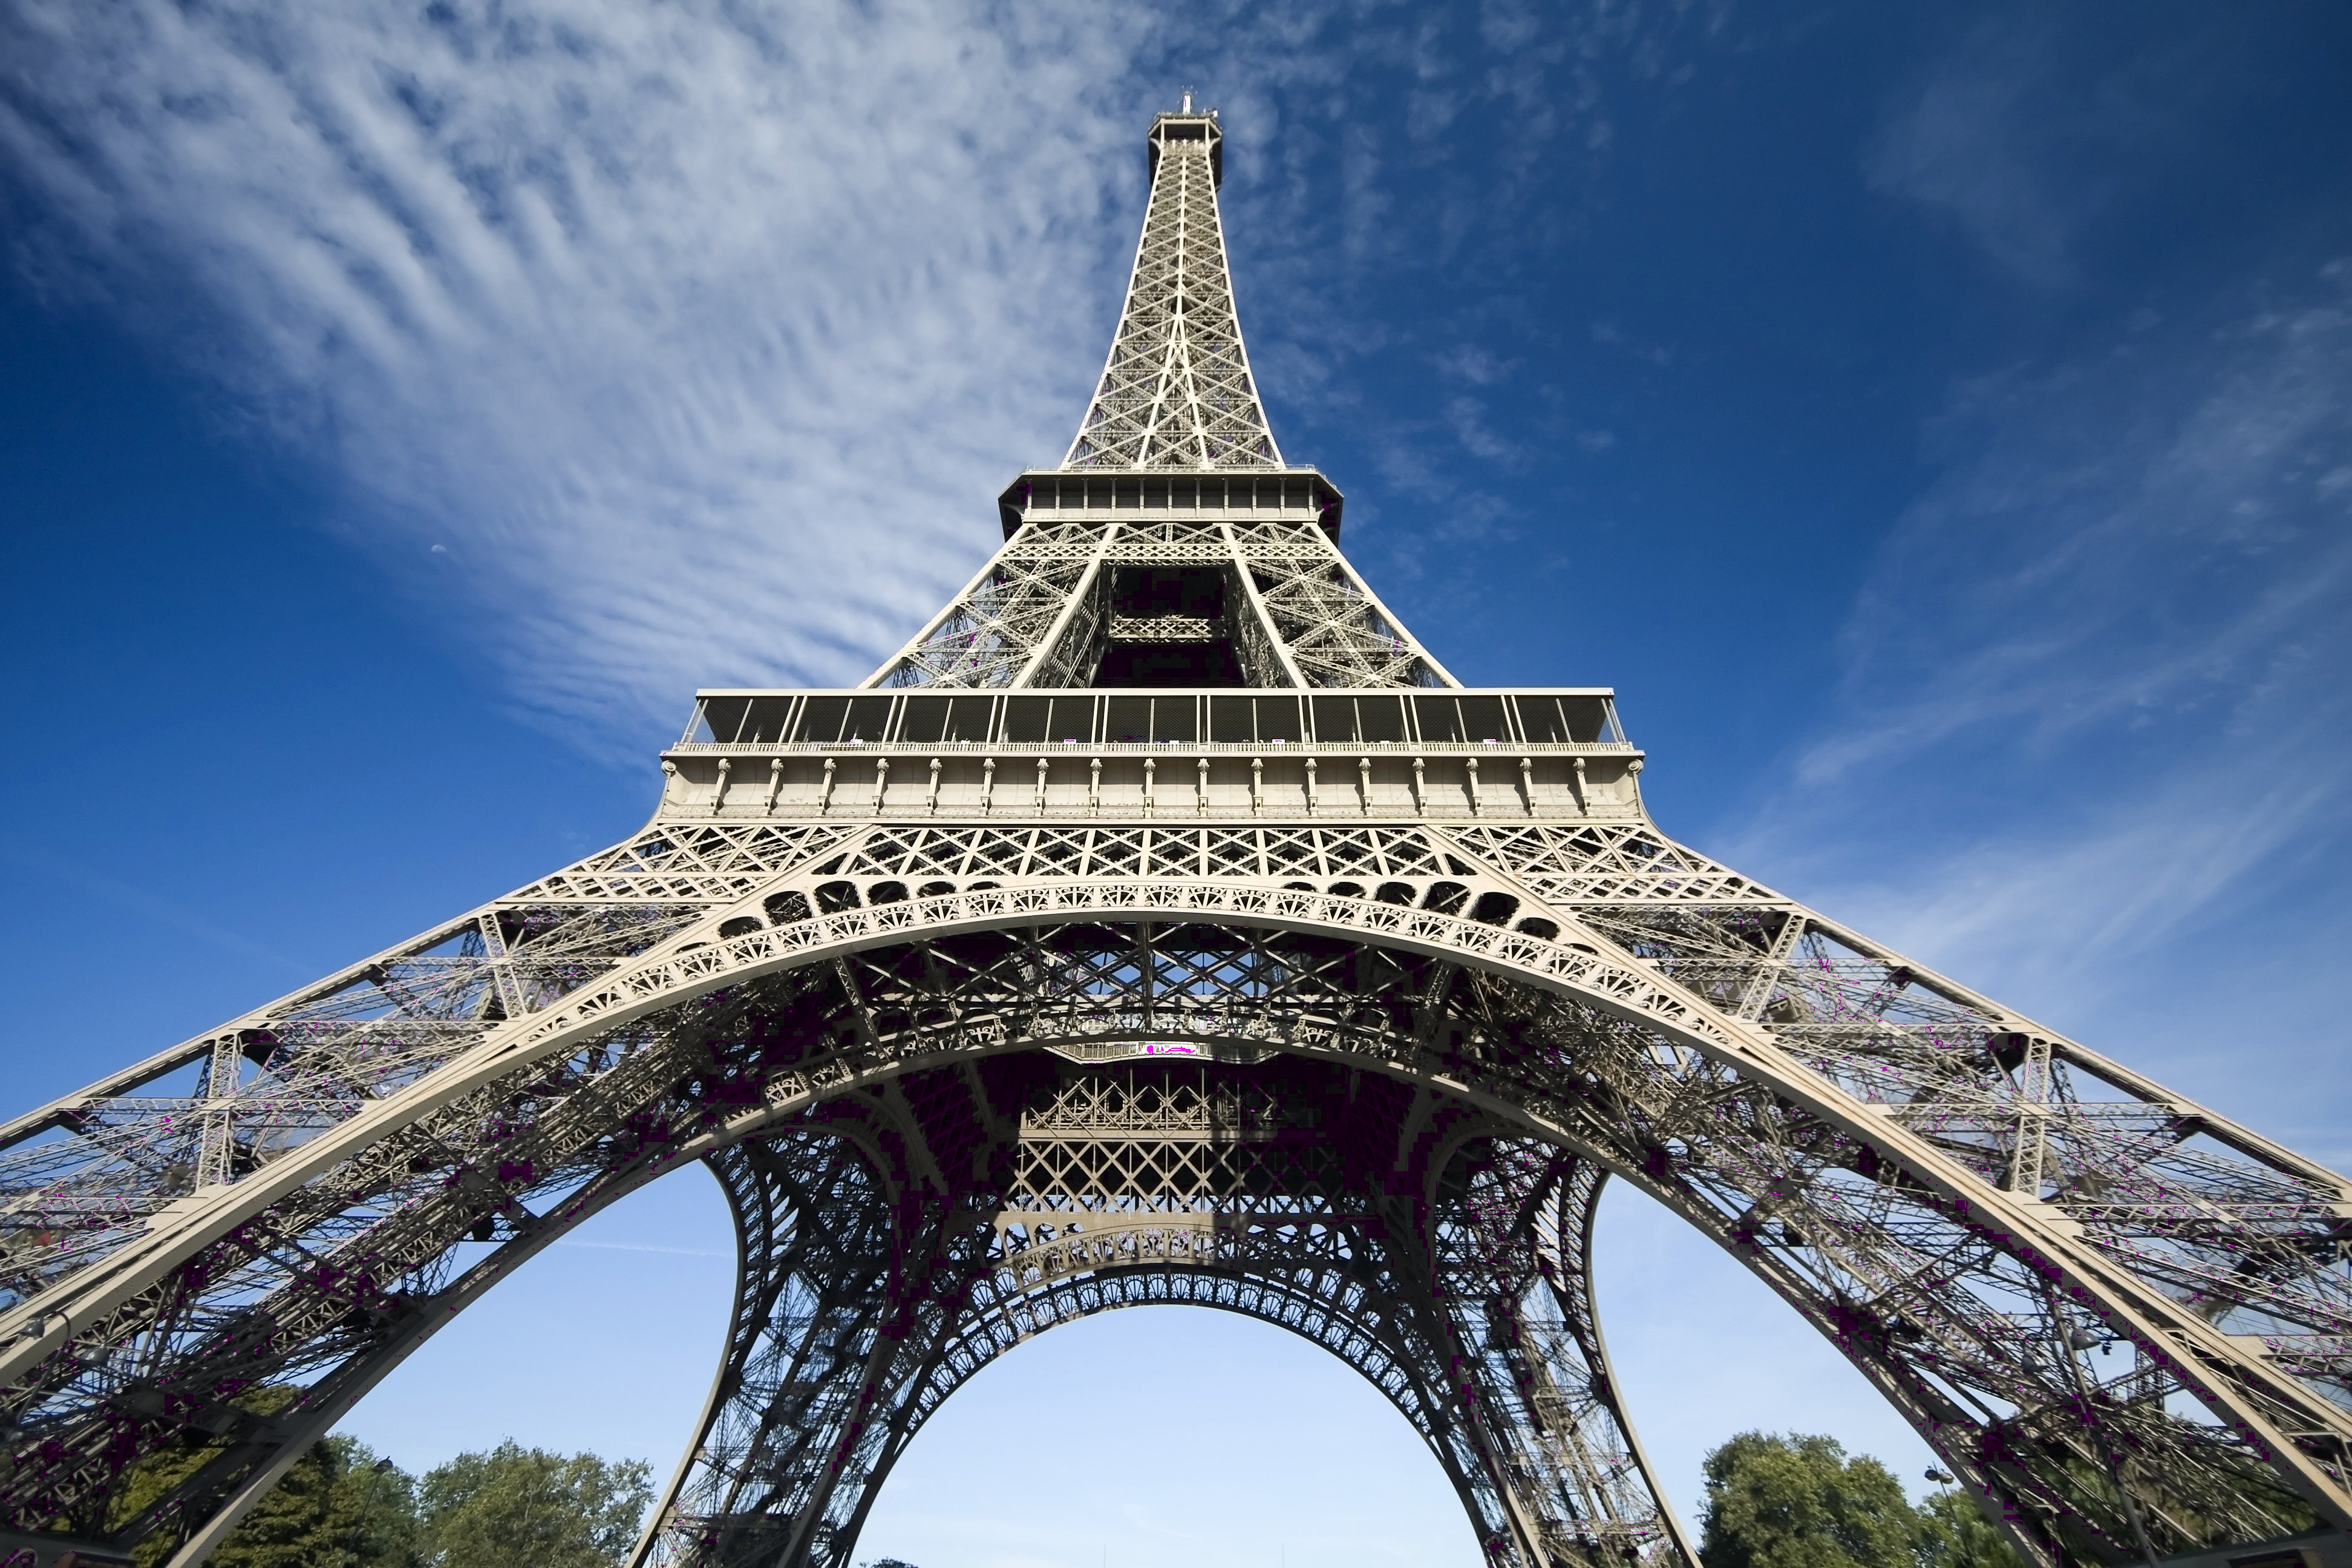
\includegraphics[width=\linewidth]{labwork8-gpu-out.jpg}
    \\
    \textit{The output image of the second part is exactly the same as the input of the labwork}
\end{center}

\section{Labwork 9: Gather}
This labwork calculates the histogram - graphical representation of the value distribution in a digital image then performs histogram equalization on grayscale image. 

Firstly, the image is converted to grayscale one then a kernel is implemented to calculate the local histogram for each column. 

\begin{lstlisting}
grayscale2d<<<gridSize, blockSize>>>(devInput, tempOutput,
        inputImage->width, inputImage->height);
histogramLocal<<<inputImage->width,1>>>(tempOutput, 
        histoLocal, inputImage->width, inputImage->height);
\end{lstlisting}

Another kernel is used to compute the final histogram of the image, which is an array of 256 integer numbers indicating the number of pixels corresponding to each value. 
\begin{lstlisting}       
histogramFinal<<<1,256>>>(histoLocal, histoFinal, 
        inputImage->width, inputImage->height);
\end{lstlisting}
Finally, the cumulative distribution function (cdf) is calculated before the normalizing process.
\begin{lstlisting}         
cdfCalculation<<<1,1>>>(histoFinal, pixelCount);
equalization<<<gridSize, blockSize>>>(tempOutput,histoFinal,
        devOutput,inputImage->width, inputImage->height);
\end{lstlisting}

\textit{Optimization:} Parameters used several times are stored in the register before calculating so it will be faster. \\

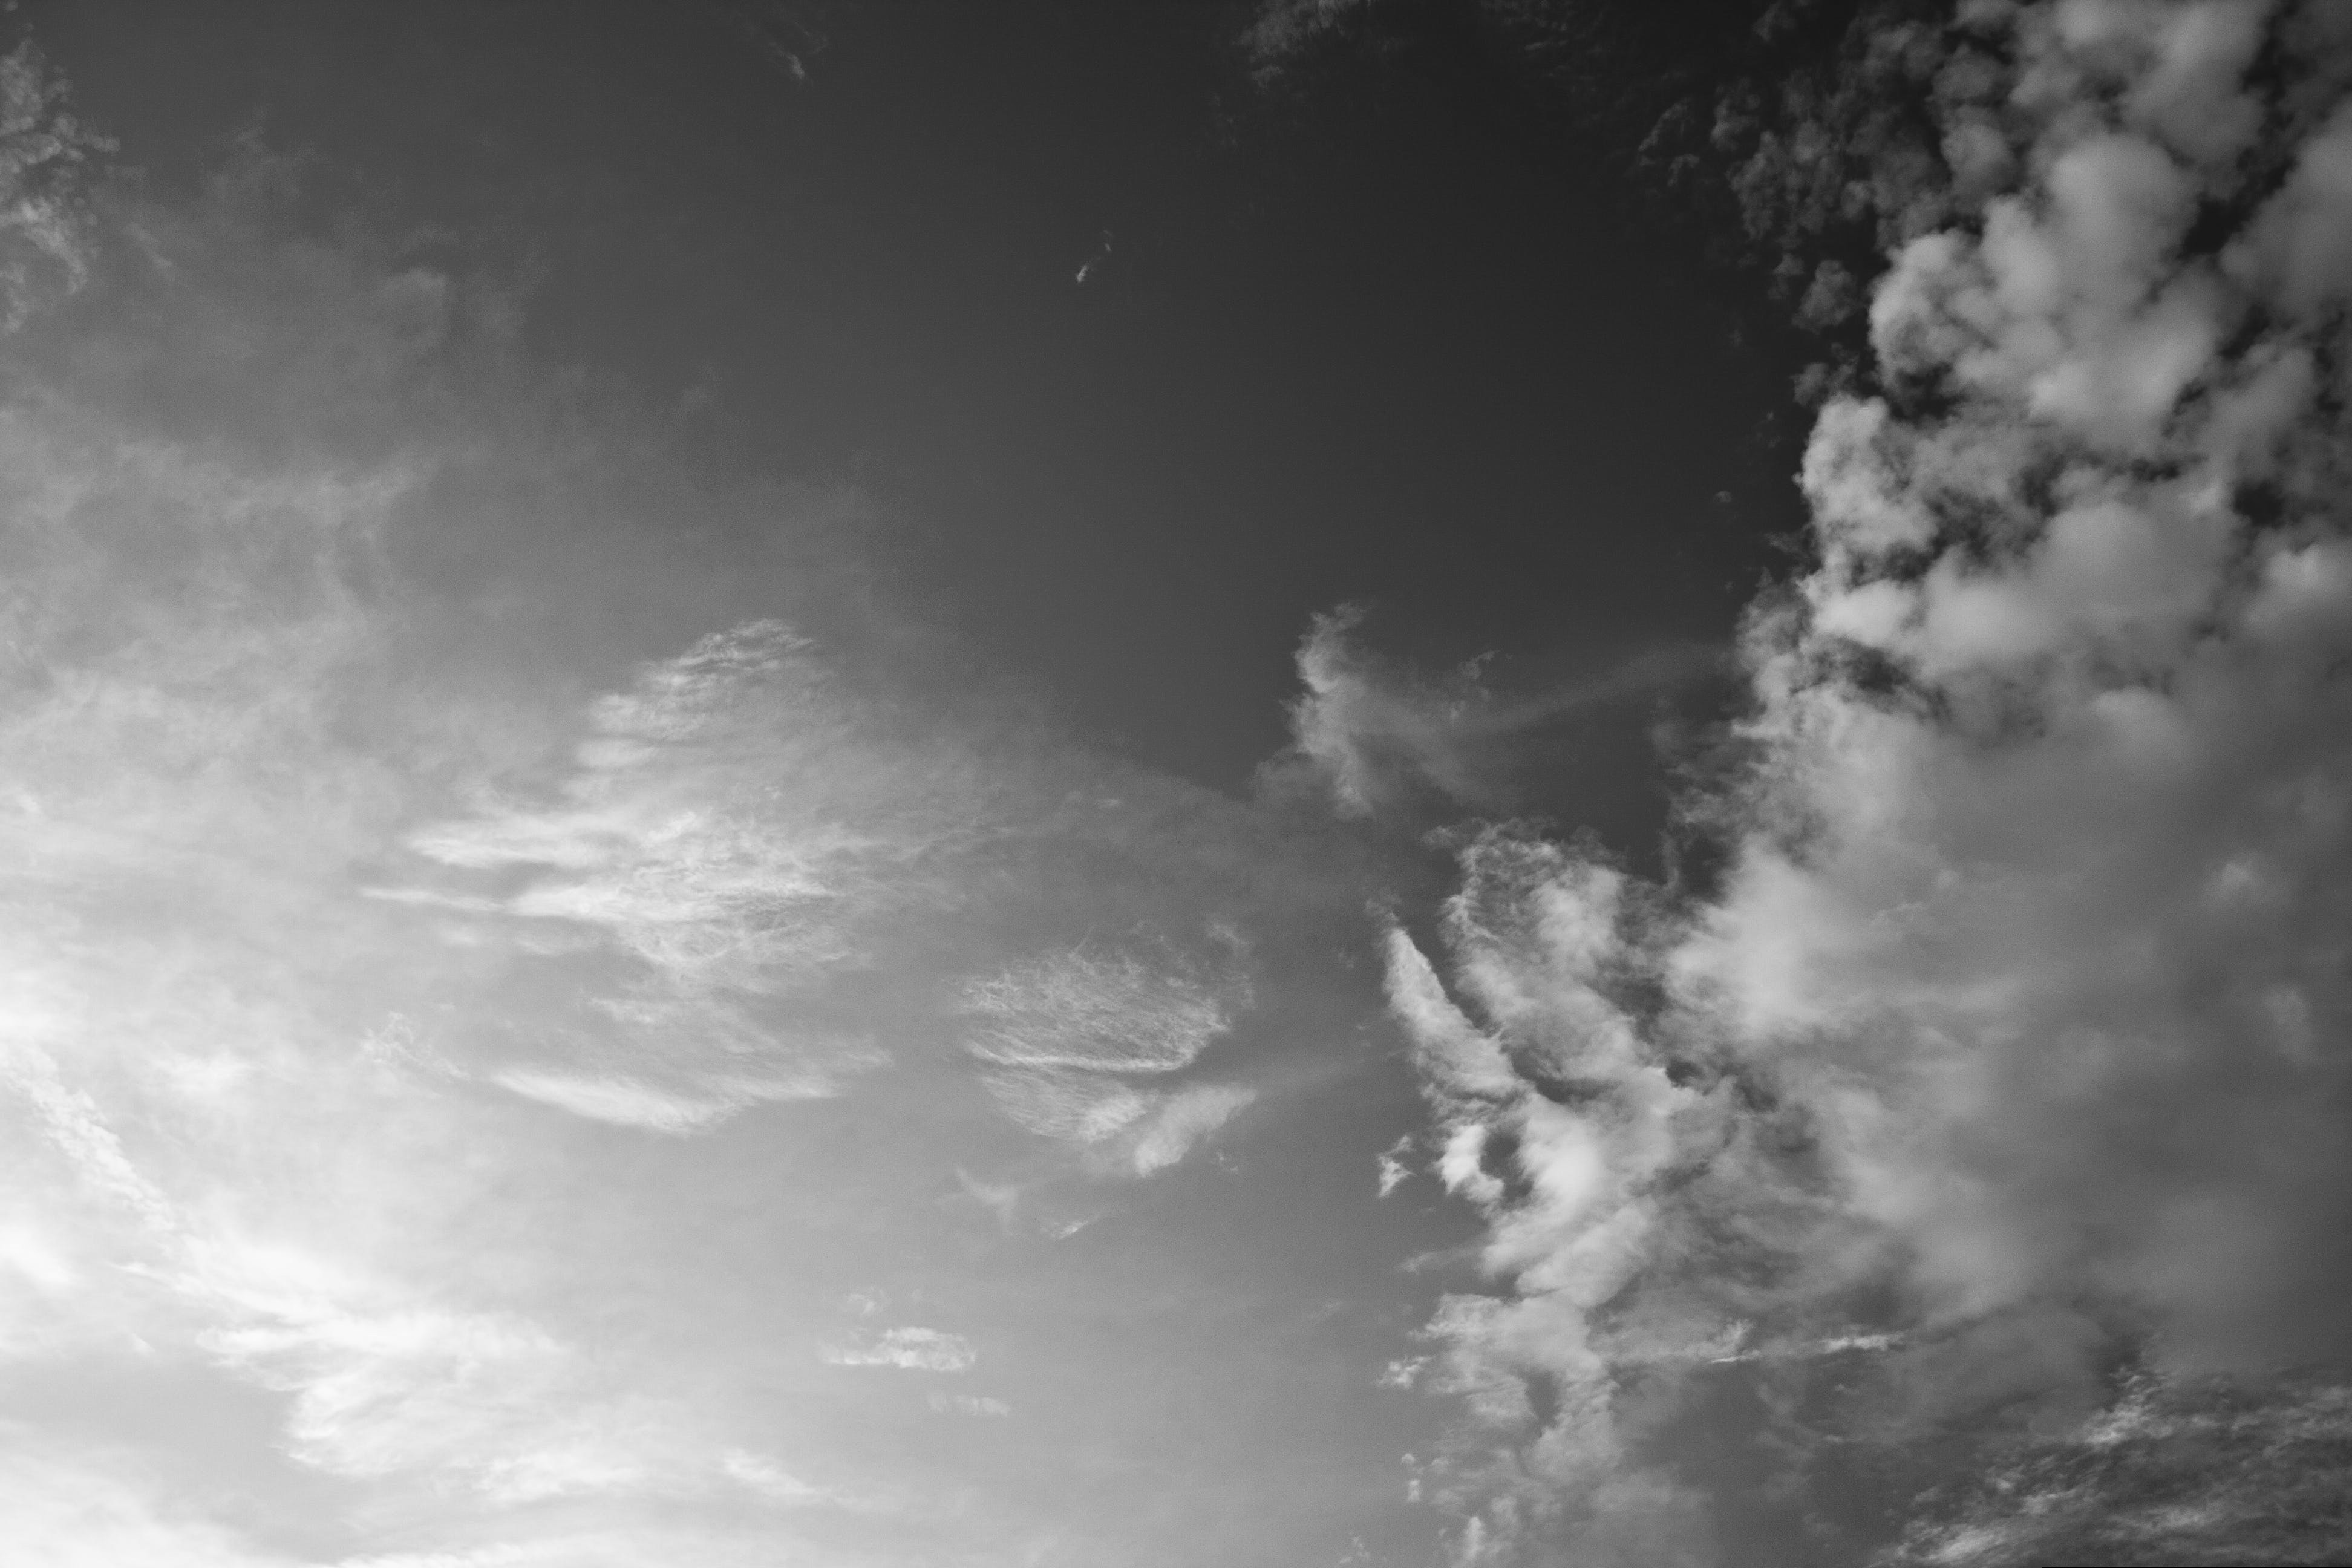
\includegraphics[scale=0.045]{skyGray.jpg}
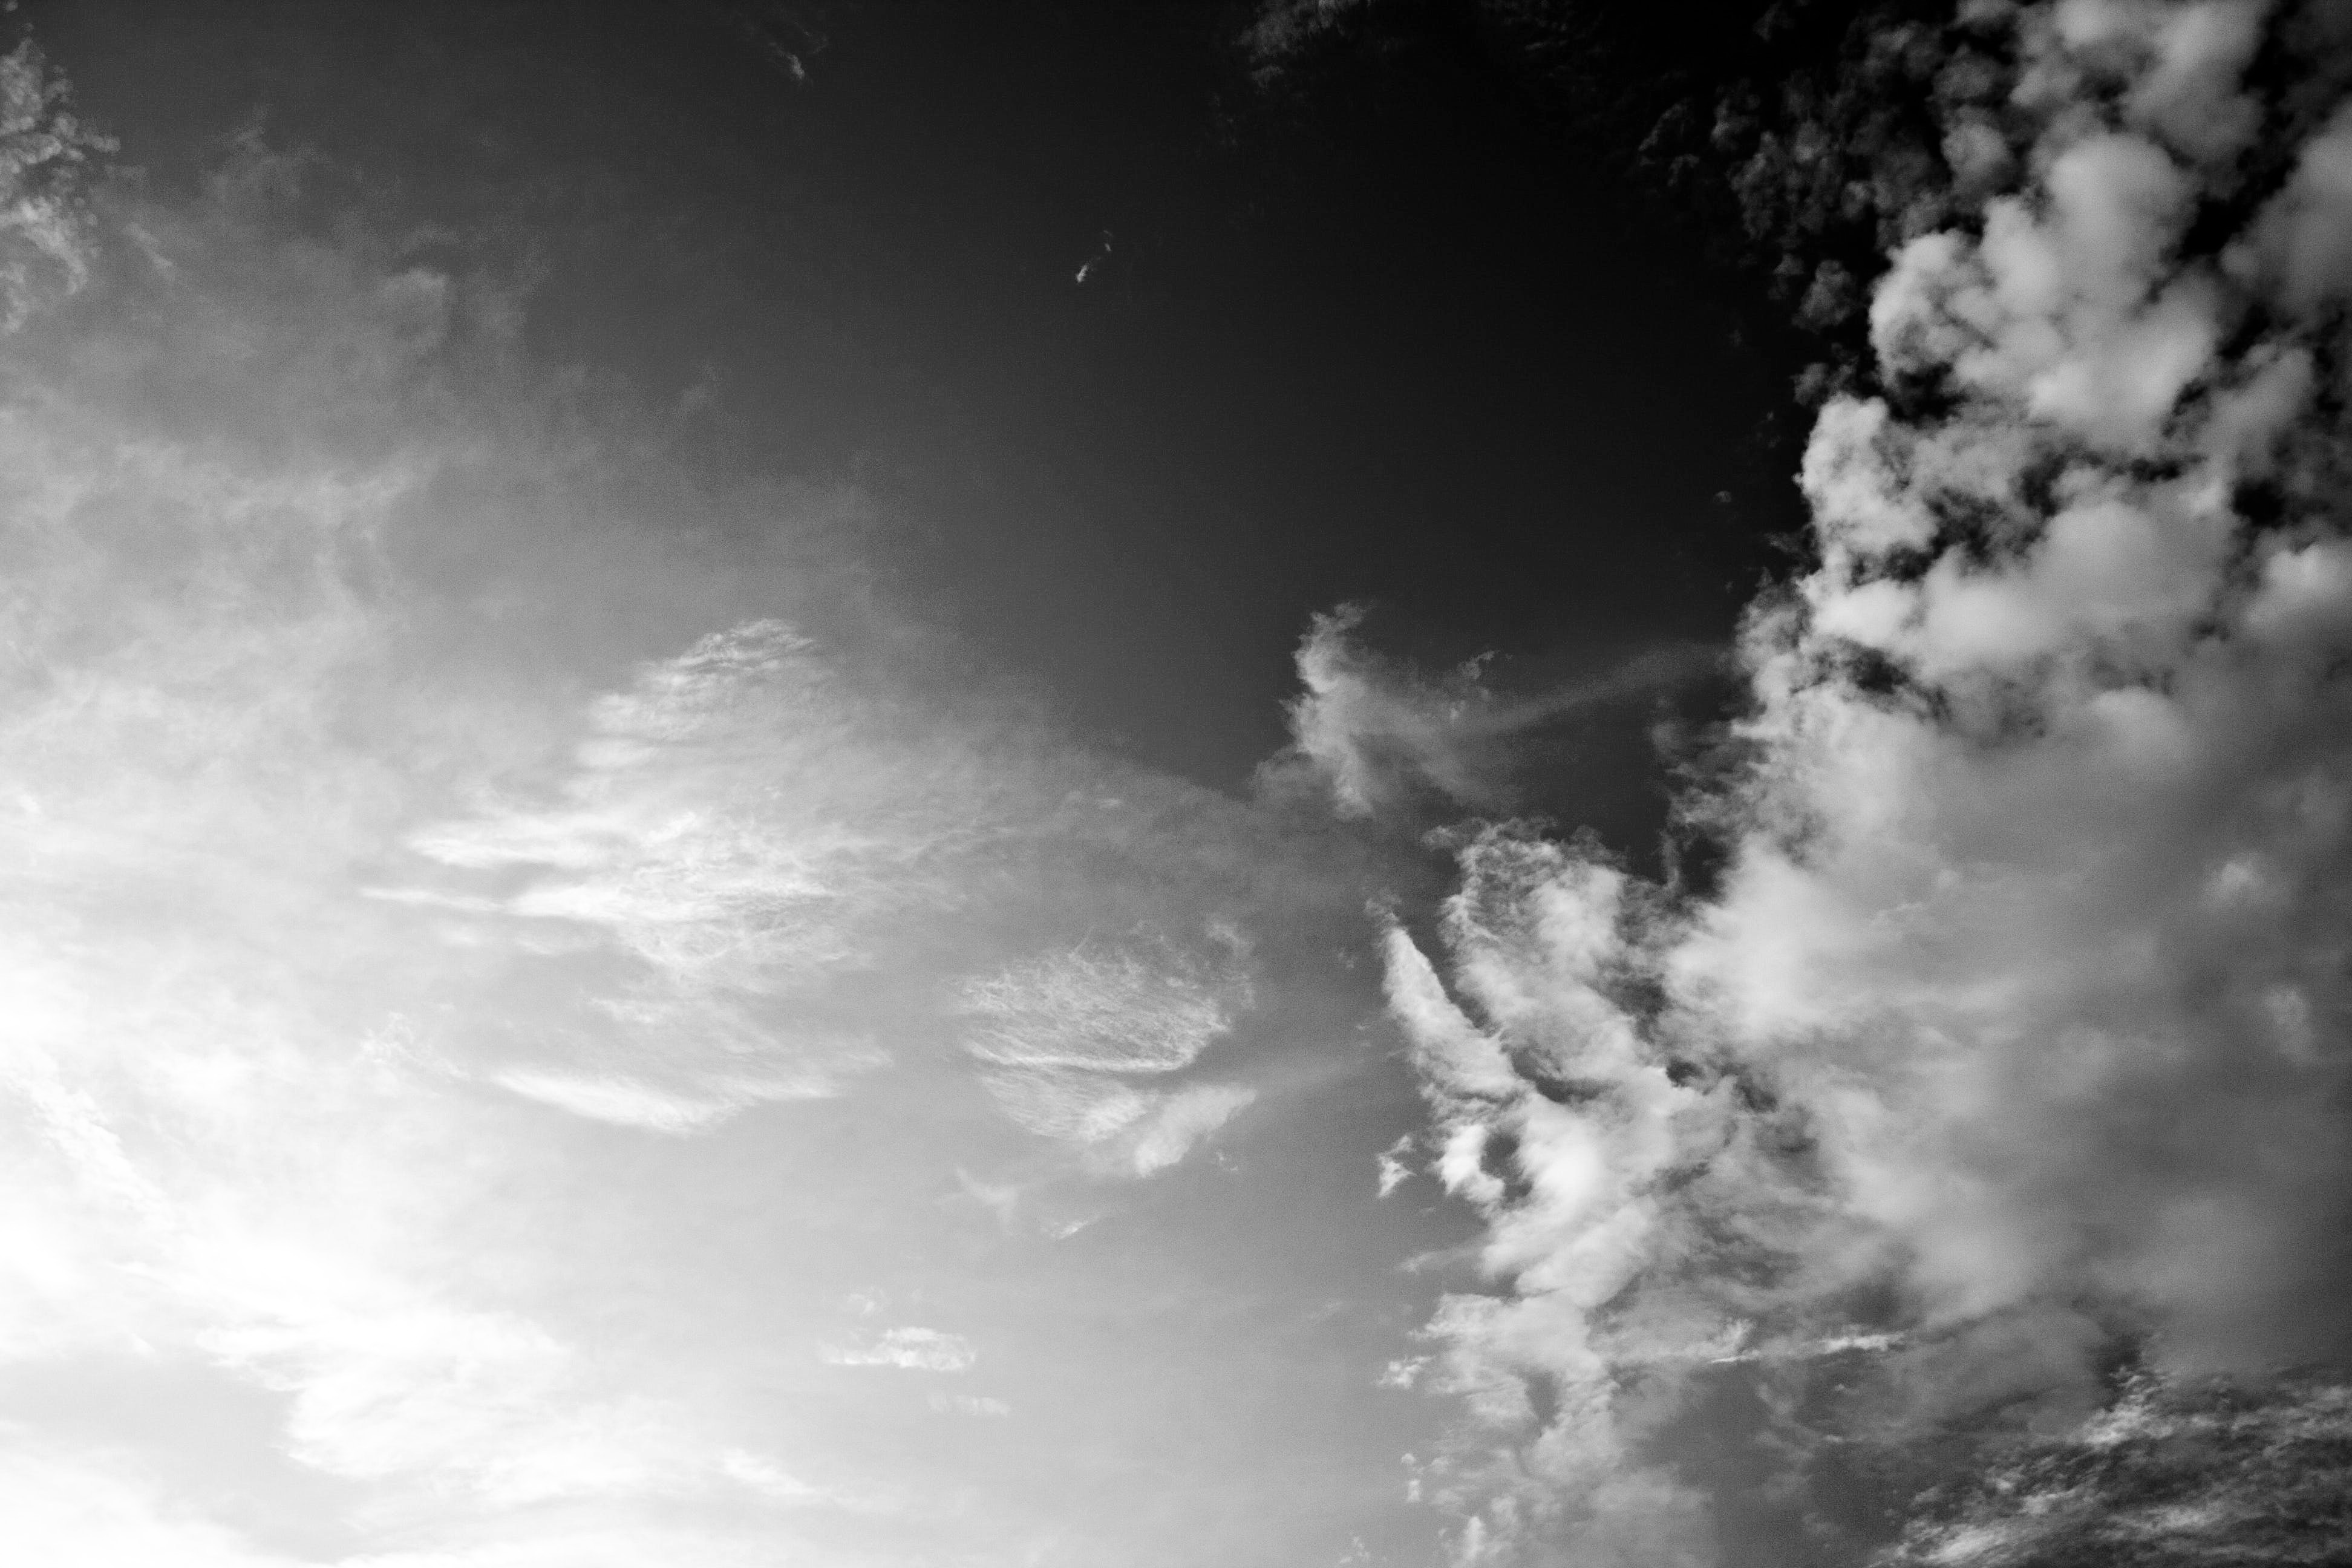
\includegraphics[scale=0.045]{labwork9-gpu-out.jpg}\\
\textit{Original grayscale image (left) and the one after normalization (right}

\section{Labwork 10: Fine-art transformation}
This labwork's task is to implement the Kuwahara filterd which can reduces noise while keeping the edge as well as produce the image oil effect.

The filter applied to each pixel is divided into 4 small windows.

\begin{lstlisting}[language=C]
        if ((x <= 0) and (y <= 0)) {
            windowPos = 0; //top left
        }
        if ((x >= 0) and (y <= 0)) {
            windowPos = 1; //top right
        }
        if ((x <= 0) and (y >= 0)) {
            windowPos = 2; //bottom left
        }
        if ((x >= 0) and (y >= 0)) {
            windowPos = 3; //bottom right
        }
\end{lstlisting}
And the mean of each window as well as the mean of each color in each window is calculated.

\begin{lstlisting}[language=C]
        for (int i = 0; i < 4; i++){
        	window[i] /= count[i];
        	for(int j = 0; j < 3; j++){ 
    		meanRGB[i][j] /= count[i];
	}	
	
\end{lstlisting}

Similarly, the standard deviation of the each window is calculated and compared to each other to find the min one.

\begin{lstlisting}[language=C]
 windowSD[windowPos] += pow((max(tempR, max(tempG,tempB)) 
                            - window[windowPos]),2.0);
        for (int i = 0; i < 4; i ++){
              windowSD[i] = sqrt(windowSD[i]/(count[i]-1));
	}	
    double minSD = min(windowSD[0], 
        min( windowSD[1], min(windowSD[2], windowSD[3])));
int windowPos;
	if (minSD == windowSD[0]) windowPos=0;
	if (minSD == windowSD[1]) windowPos=1;
	if (minSD == windowSD[2]) windowPos=2;
	if (minSD == windowSD[3]) windowPos=3;
\end{lstlisting}
 Then the output color value of the pixel will be equal to mean color value of the window that has the smallest standard deviation.

\begin{lstlisting}[language=C]
        output[tid].x = meanRGB[windowPos][0];
	output[tid].y = meanRGB[windowPos][1];
	output[tid].z = meanRGB[windowPos][2];
\end{lstlisting}

\textit{Optimization:} Parameters used several times are stored in the register before calculating so it will be faster. \\

\begin{center}
    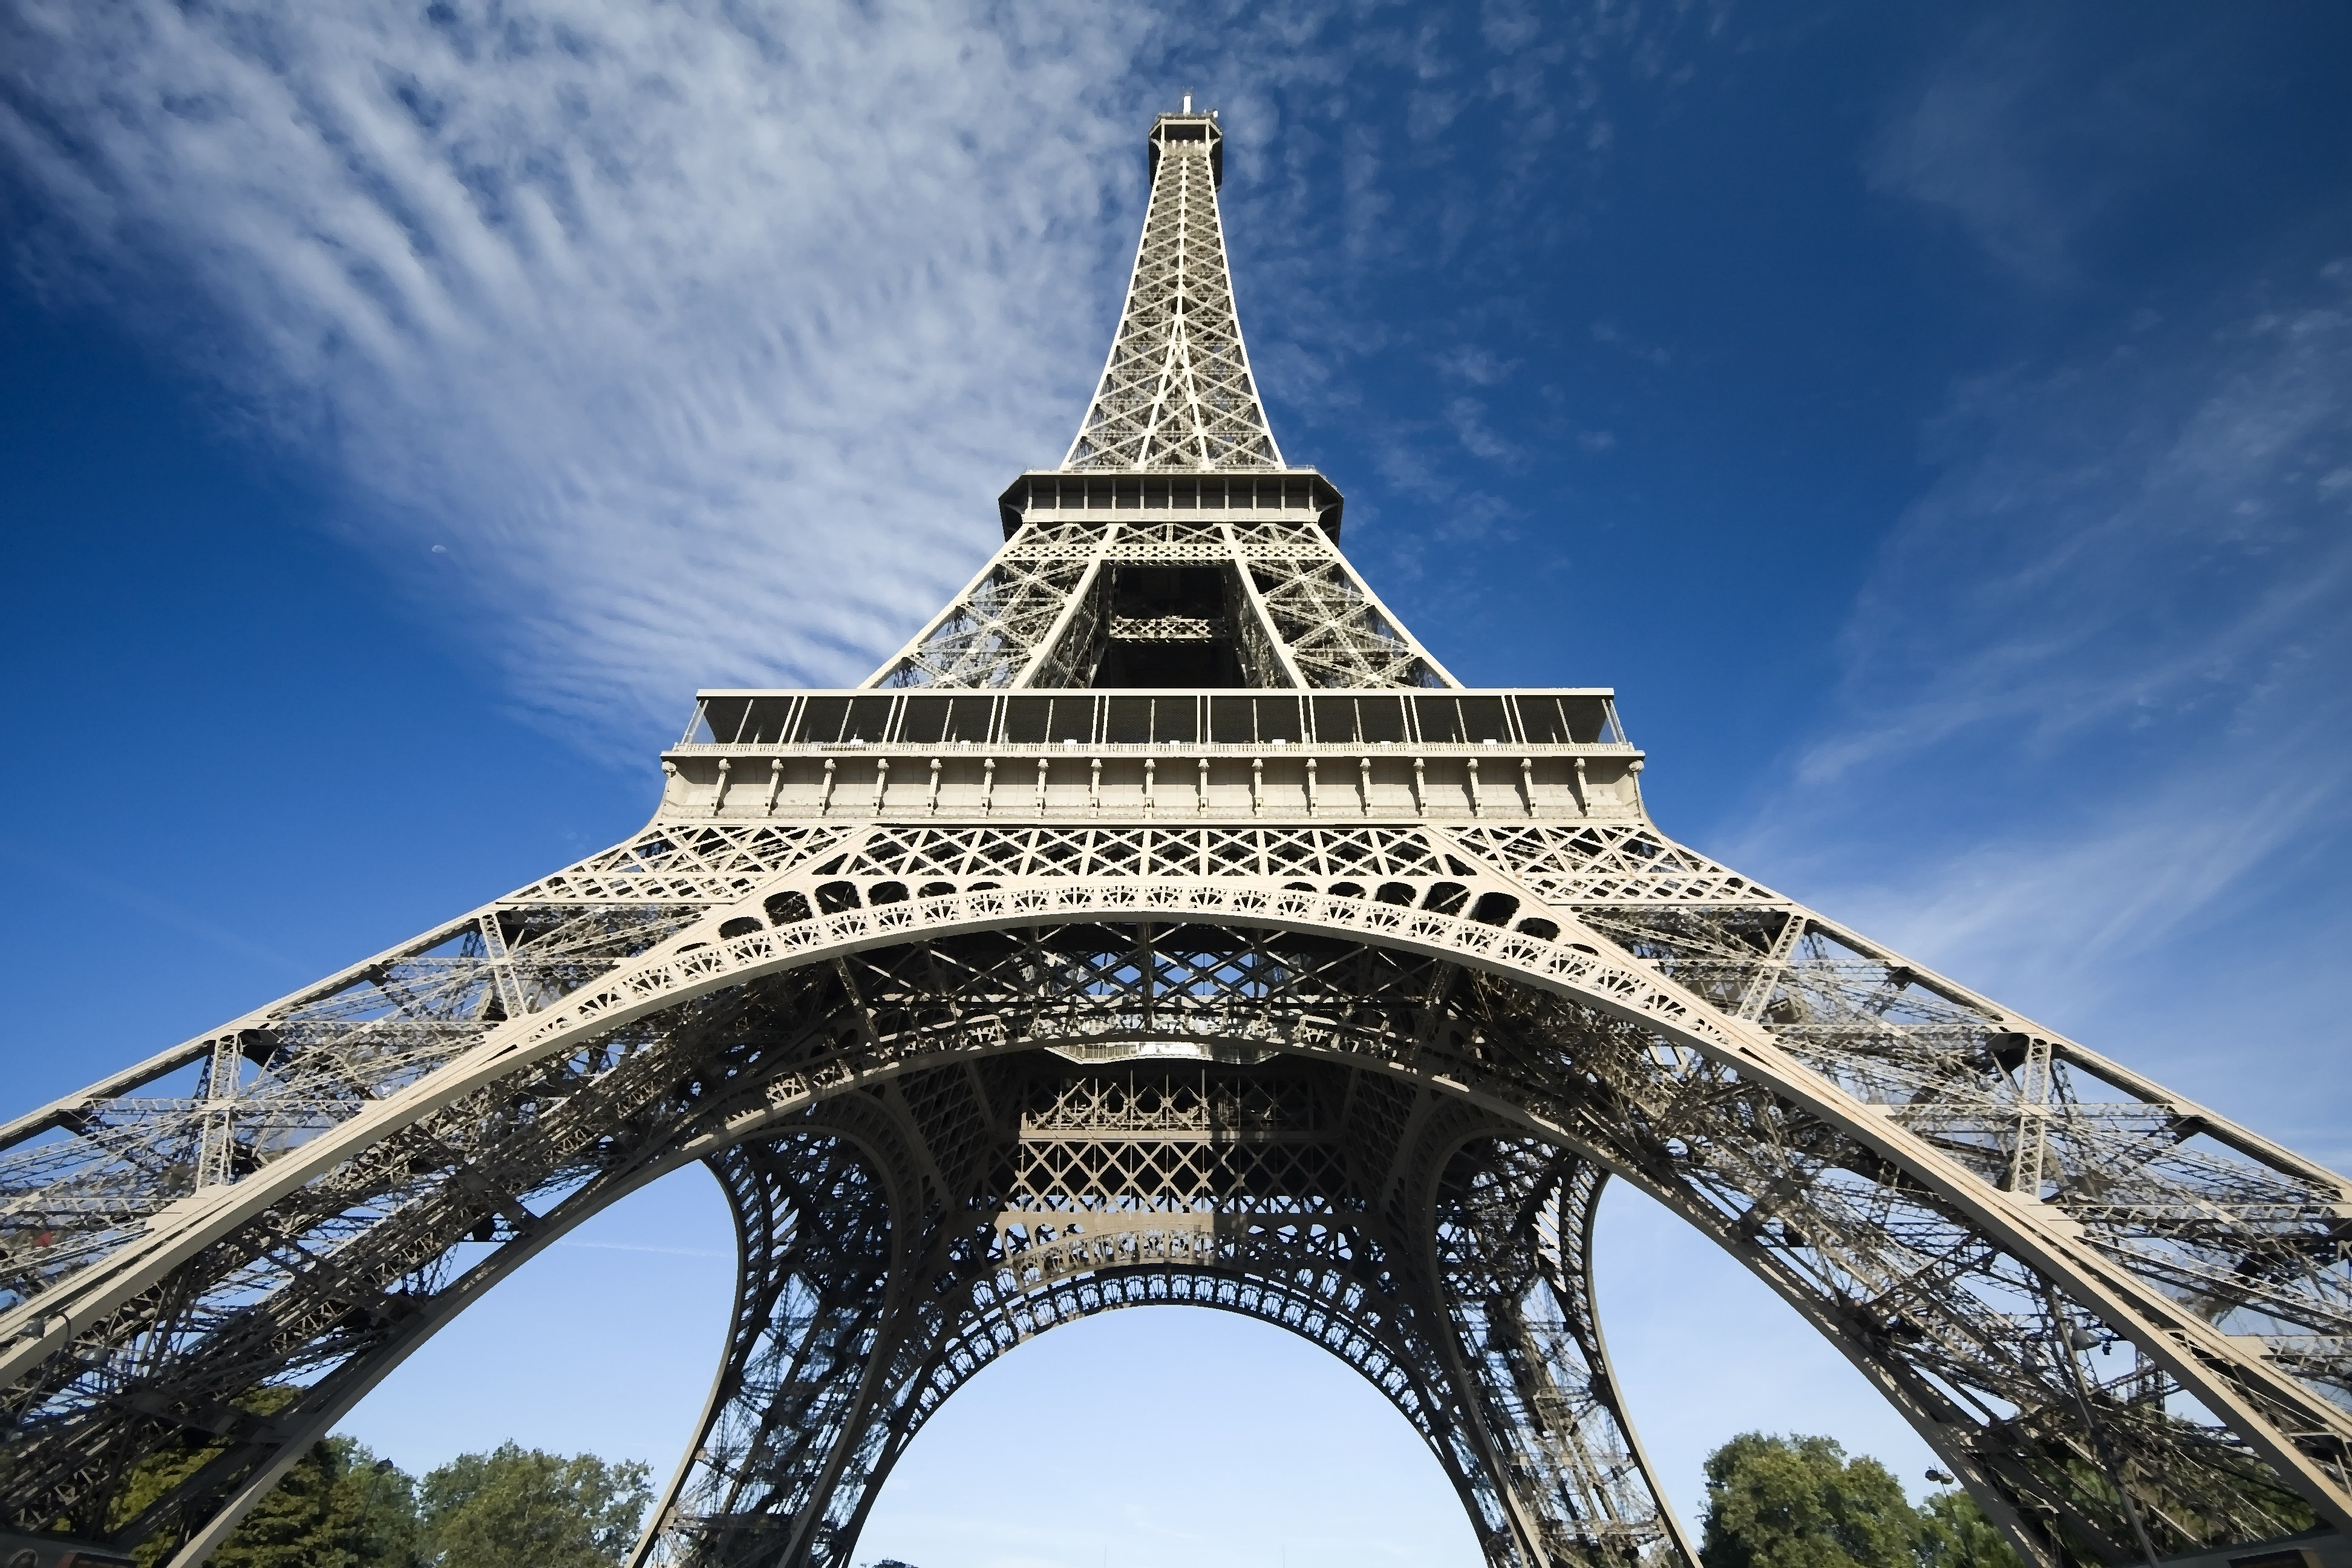
\includegraphics[width=\linewidth]{kuwahara.jpg}
    \\
    \textit{Eiffel image after Kuwahara filtering with window size = 3}
\end{center}

\begin{center}
    \includegraphics[width=\linewidth]{compare.png}
    \\
    \textit{Compare the original image with the Kuwahara filtered one}
\end{center}

\end{document}
